%\documentclass[first,firstsupp,handout,compress,notes,navigation,hyperref,table]{ETHclass}
%\documentclass[first,firstsupp,handout,lastsupp]{ETHclass}
\documentclass[first,firstsupp,lastsupp,last,hyperref,table]{ETHclass}
%\documentclass[first,firstsupp]{ETHclass}
\usepackage{etex}


\usepackage{adjustbox}
\usepackage{amsmath}
\usepackage{amssymb}
\usepackage{animate}
\usepackage{booktabs}
\usepackage{charter}
\usepackage{enumitem}
\usepackage{etoolbox}
\usepackage{ifthen}
\usepackage{longtable}
\usepackage{mathrsfs}
\usepackage{multicol}
\usepackage{pgf}
\usepackage{pgfpages}
\usepackage{pgfplots}
\usepackage{pifont}
\usepackage{ragged2e}
\usepackage{standalone}
\usepackage[caption=false]{subfig}
\usepackage{tabularx}
\usepackage{tikz}
\usepackage{verbatim}
\usepackage{xcolor}
\usepackage{hyperref}

\pgfplotsset{compat=1.7}

\setbeamertemplate{navigation symbols}{}
\usetikzlibrary{arrows,decorations.pathreplacing,positioning,shapes,shadows}

%\usepackage[style=numeric-comp]{biblatex}

%\usepackage{lipsum}

%\usetikzlibrary{fit}
\usetikzlibrary{arrows}
\usetikzlibrary{trees}

% Options for beamer:
%
% 9,10,11,12,13,14,17pt  Fontsizes
%
% compress: navigation bar becomes smaller
% t       : place contents of frames on top (alternative: b,c)
% handout : handoutversion
% notes   : show notes
% notes=onlyslideswithnotes
%
%hyperref={bookmarksopen,bookmarksnumbered} : Needed for menues in
%                                             acrobat. Also need
%                                             pdftex as option or
%                                             compile with
% pdflatex '\PassOptionsToPackage{pdftex,bookmarksopen,bookmarksnumbered}{hyperref} \input{file}'

%\usepackage{beamerseminar}
%\usepackage[accumulated]{beamerseminar}
                                % remove ``accumulated'' option
                                % for original behaviour
%\usepackage{beamerbasenotes}
%\setbeamertemplate{note page}[plain]
%\setbeameroption{notes on second screen}

%\setbeamertemplate{note page}[plain]
%\setbeamertemplate{note page}{\ \\[.3cm]
%\textbf{\color{blue}Notes:}\\%[0.1cm]
%{\footnotesize %\tiny
%\insertnote}}
%\setbeameroption{notes on second screen}


\setbeamertemplate{navigation symbols}{} % suppresses all navigation symbols:
% \setbeamertemplate{navigation symbols}[horizontal] % Organizes the navigation symbols horizontally.
 %\setbeamertemplate{navigation symbols}[vertical] % Organizes the navigation symbols vertically.
% \setbeamertemplate{navigation symbols}[only frame symbol] % Shows only the navigational symbol for navigating frames.

\setlayoutscale{0.5}
\setparametertextfont{\scriptsize}
\setlabelfont{\scriptsize}

% \useoutertheme[subsection=false]{miniframes}
% \usepackage{etoolbox}
% \makeatletter
% \patchcmd{\slideentry}{\advance\beamer@xpos by1\relax}{}{}{}
% \def\beamer@subsectionentry#1#2#3#4#5{\advance\beamer@xpos by1\relax}%
% \makeatother

% \makeatletter
%     \newenvironment{withoutheadline}{
%        \setbeamertemplate{headline}{%
% \vspace{15pt}
% }
%     }{}
% \makeatother

\makeatletter
    \newenvironment{withoutheadline}{
         \setbeamertemplate{headline}{%
\vspace{35pt}
}
        %\def\beamer@entrycode{\vspace*{-1.5\headheight}}
    }{}
\makeatother

\newcommand{\Cross}{$\mathbin{\tikz [x=1.4ex,y=1.4ex,line width=.2ex, red] \draw (0,0) -- (1,1) (0,1) -- (1,0);}$}%

\newcommand{\Checkmark}{$\color{green}\checkmark$}

\setbeamerfont{subsection in toc}{size=\tiny}

\makeatletter
\patchcmd{\beamer@sectionintoc}
  {\vfill}
  {\vskip1.5\itemsep}
  {}
  {}
\makeatother

\setbeamertemplate{frametitle continuation}{}

\setbeamertemplate{bibliography entry title}{}
\setbeamertemplate{bibliography entry author}{}
\setbeamertemplate{bibliography entry location}{}
\setbeamertemplate{bibliography entry note}{}

\setbeamercolor*{bibliography entry title}{fg=black}
\setbeamercolor*{bibliography entry author}{fg=black}
\setbeamercolor*{bibliography entry location}{fg=black}
\setbeamercolor*{bibliography entry note}{fg=black}
% and kill the abominable icon
%\setbeamertemplate{bibliography item}{\color{forestgreen}$\blacktriangleright$}
\setbeamertemplate{bibliography item}{\insertbiblabel}
%\setbeamertemplate{bibliography item}{\theenumiv}

\newcommand{\highlightred}[1]{%
  \colorbox{red!50}{$\displaystyle#1$}}

\newcommand{\highlightyellow}[1]{%
  \colorbox{yellow!50}{$\displaystyle#1$}}

\newcommand{\highlightgreen}[1]{%
  \colorbox{green!50}{$\displaystyle#1$}}

\AtBeginSection[]{
  \begin{frame}
  \vfill
  \centering
  \begin{beamercolorbox}[sep=8pt,center,shadow=true,rounded=true]{title}
    \usebeamerfont{frametitle}
\includegraphics[width=2ex]{freccia_trasparente_verde_foresta.png}\hspace{.5ex}~{\LARGE \textsc{\bfseries \insertsectionhead}}\par%
  \end{beamercolorbox}
  \vfill
  \end{frame}
}

\hyphenpenalty=5000
\tolerance=1000

\graphicspath{{figures/}}

\newenvironment{system}{\left\lbrace\begin{array}{@{}l@{}}}{\end{array}\right.}

\newenvironment{subsystem}{\left\lgroup\begin{array}{@{}l@{}}}{\end{array}\right.}

\defbeamertemplate*{title page}{customized}[1][]
{
\usebeamerfont{subtitle}
\usebeamercolor[fg]{subtitle}

\vspace{-1.75cm}

{\flushleft
 \usebeamerfont{title}{\inserttitle}\par
}
\vspace{-.25cm}
{\flushleft
 \usebeamerfont{subtitle}{\small \insertsubtitle} \par
}

%\vspace{-.5cm}

{\flushright
\setbeamercolor{author}{bg=white,fg=Red}
\usebeamerfont{author}{\footnotesize \insertauthor} \par}

\vspace{-.2cm}

{\flushright
\usebeamerfont{institute}{\tiny \insertinstitute}\par }

\vspace{.2cm}

{\centering
\usebeamerfont{date}{\scriptsize \insertdate} \par }

\vspace{0.2in}
}


\begin{document}
\setbeamertemplate{caption}{\raggedright\insertcaption\par}

\title[\textsc{FEM \& the Fiber-Matrix Interface Crack}]{\textsc{The Fiber-Matrix Interface Crack Problem and its Solution by the Finite Element Method}}
\author{ \underline{L. Di Stasio}$^{1,2}$, Z. Ayadi$^{1}$, J. Varna$^{2}$}
%\institute{ Science et Ing\'enierie des Mat\'eriaux et M\'etallurgie (SI2M), Institut Jean Lamour, Nancy, France\\Department of Engineering Sciences and Mathematics, Division of Materials Science, Lule\aa\ University of Technology, Lule\aa, Sweden}
\institute{$^{1}$EEIGM \& IJL, Universit\'e de Lorraine, Nancy, France\\$^{2}$Division of Materials Science, Lule\aa\ University of Technology, Lule\aa, Sweden}
\date{Mid-Term Defence - Nancy (FR), October 24, 2017}

\begin{frame}[plain]
    \titlepage

\end{frame}

\begin{withoutheadline}
\begin{frame}
\frametitle{Outline}
\justifying
\vspace*{-0.5cm}
% \tableofcontents[hidesubsections]
% \begin{multicols}{2}
% \tableofcontents[hidesubsections]
% \end{multicols}
% \begin{columns}[t]
%         \begin{column}{.5\textwidth}
%             \tableofcontents[sections={1-2}]
%         \end{column}
%         \begin{column}{.5\textwidth}
%             \tableofcontents[sections={3-6}]
%         \end{column}
%     \end{columns}
% \end{frame}
\tableofcontents[hidesubsections]
\end{frame}
\end{withoutheadline}

%\note{}

%\begin{frame}
%\pagediagram
%\end{frame}
%% \note{}

\section[Damage in Thin Ply FRPC]{Damage Mechanisms in Thin Ply Fiber Reinforced Polymer Laminates}

\subsection{Spread Tow Technology}

\begin{frame}
\frametitle{\small Spread Tow Technology: Introduction}
\vspace{-0.25cm}
\centering
\begin{itemize}[label=\ding{212}]
	\item {\small Firstly developed for commercial use in Japan between 1995 and 1998 (Kawabe, Tomoda et al. 1997 [1], 2003 [2], 2008 [3], 2009 [4])}
	\item {\small In the last decade its use has been spreading, from sports' equipments to mission-critical applications as in the \textit{Solar Impulse 2}}
	\item {\small Only a few producers wolrdwide: NTPT (USA-CH) [5], Oxeon (SE) [6], Chomarat (FR), Hexcel (USA), Technomax (JP)}
\end{itemize}
\begin{figure}[!h]
\centering
\subfloat[\scriptsize By North Thin Ply Technology.\label{fig:solar_impulse}]{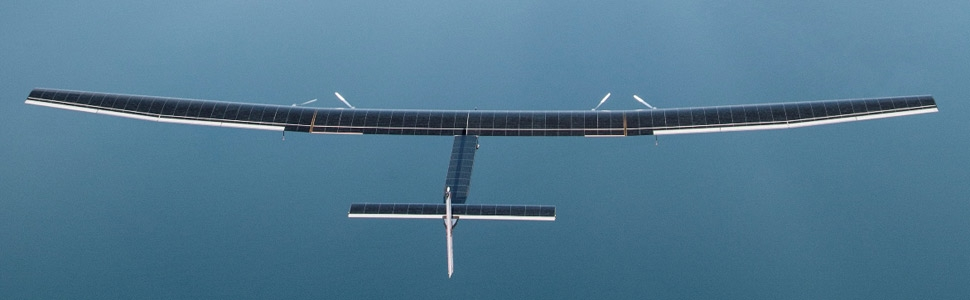
\includegraphics[height=0.25\textheight,width=0.45\textwidth]{ntpt_solar-impulse-1.jpg}}\quad
\subfloat[\scriptsize By TeXtreme.\label{fig:solar_car}]{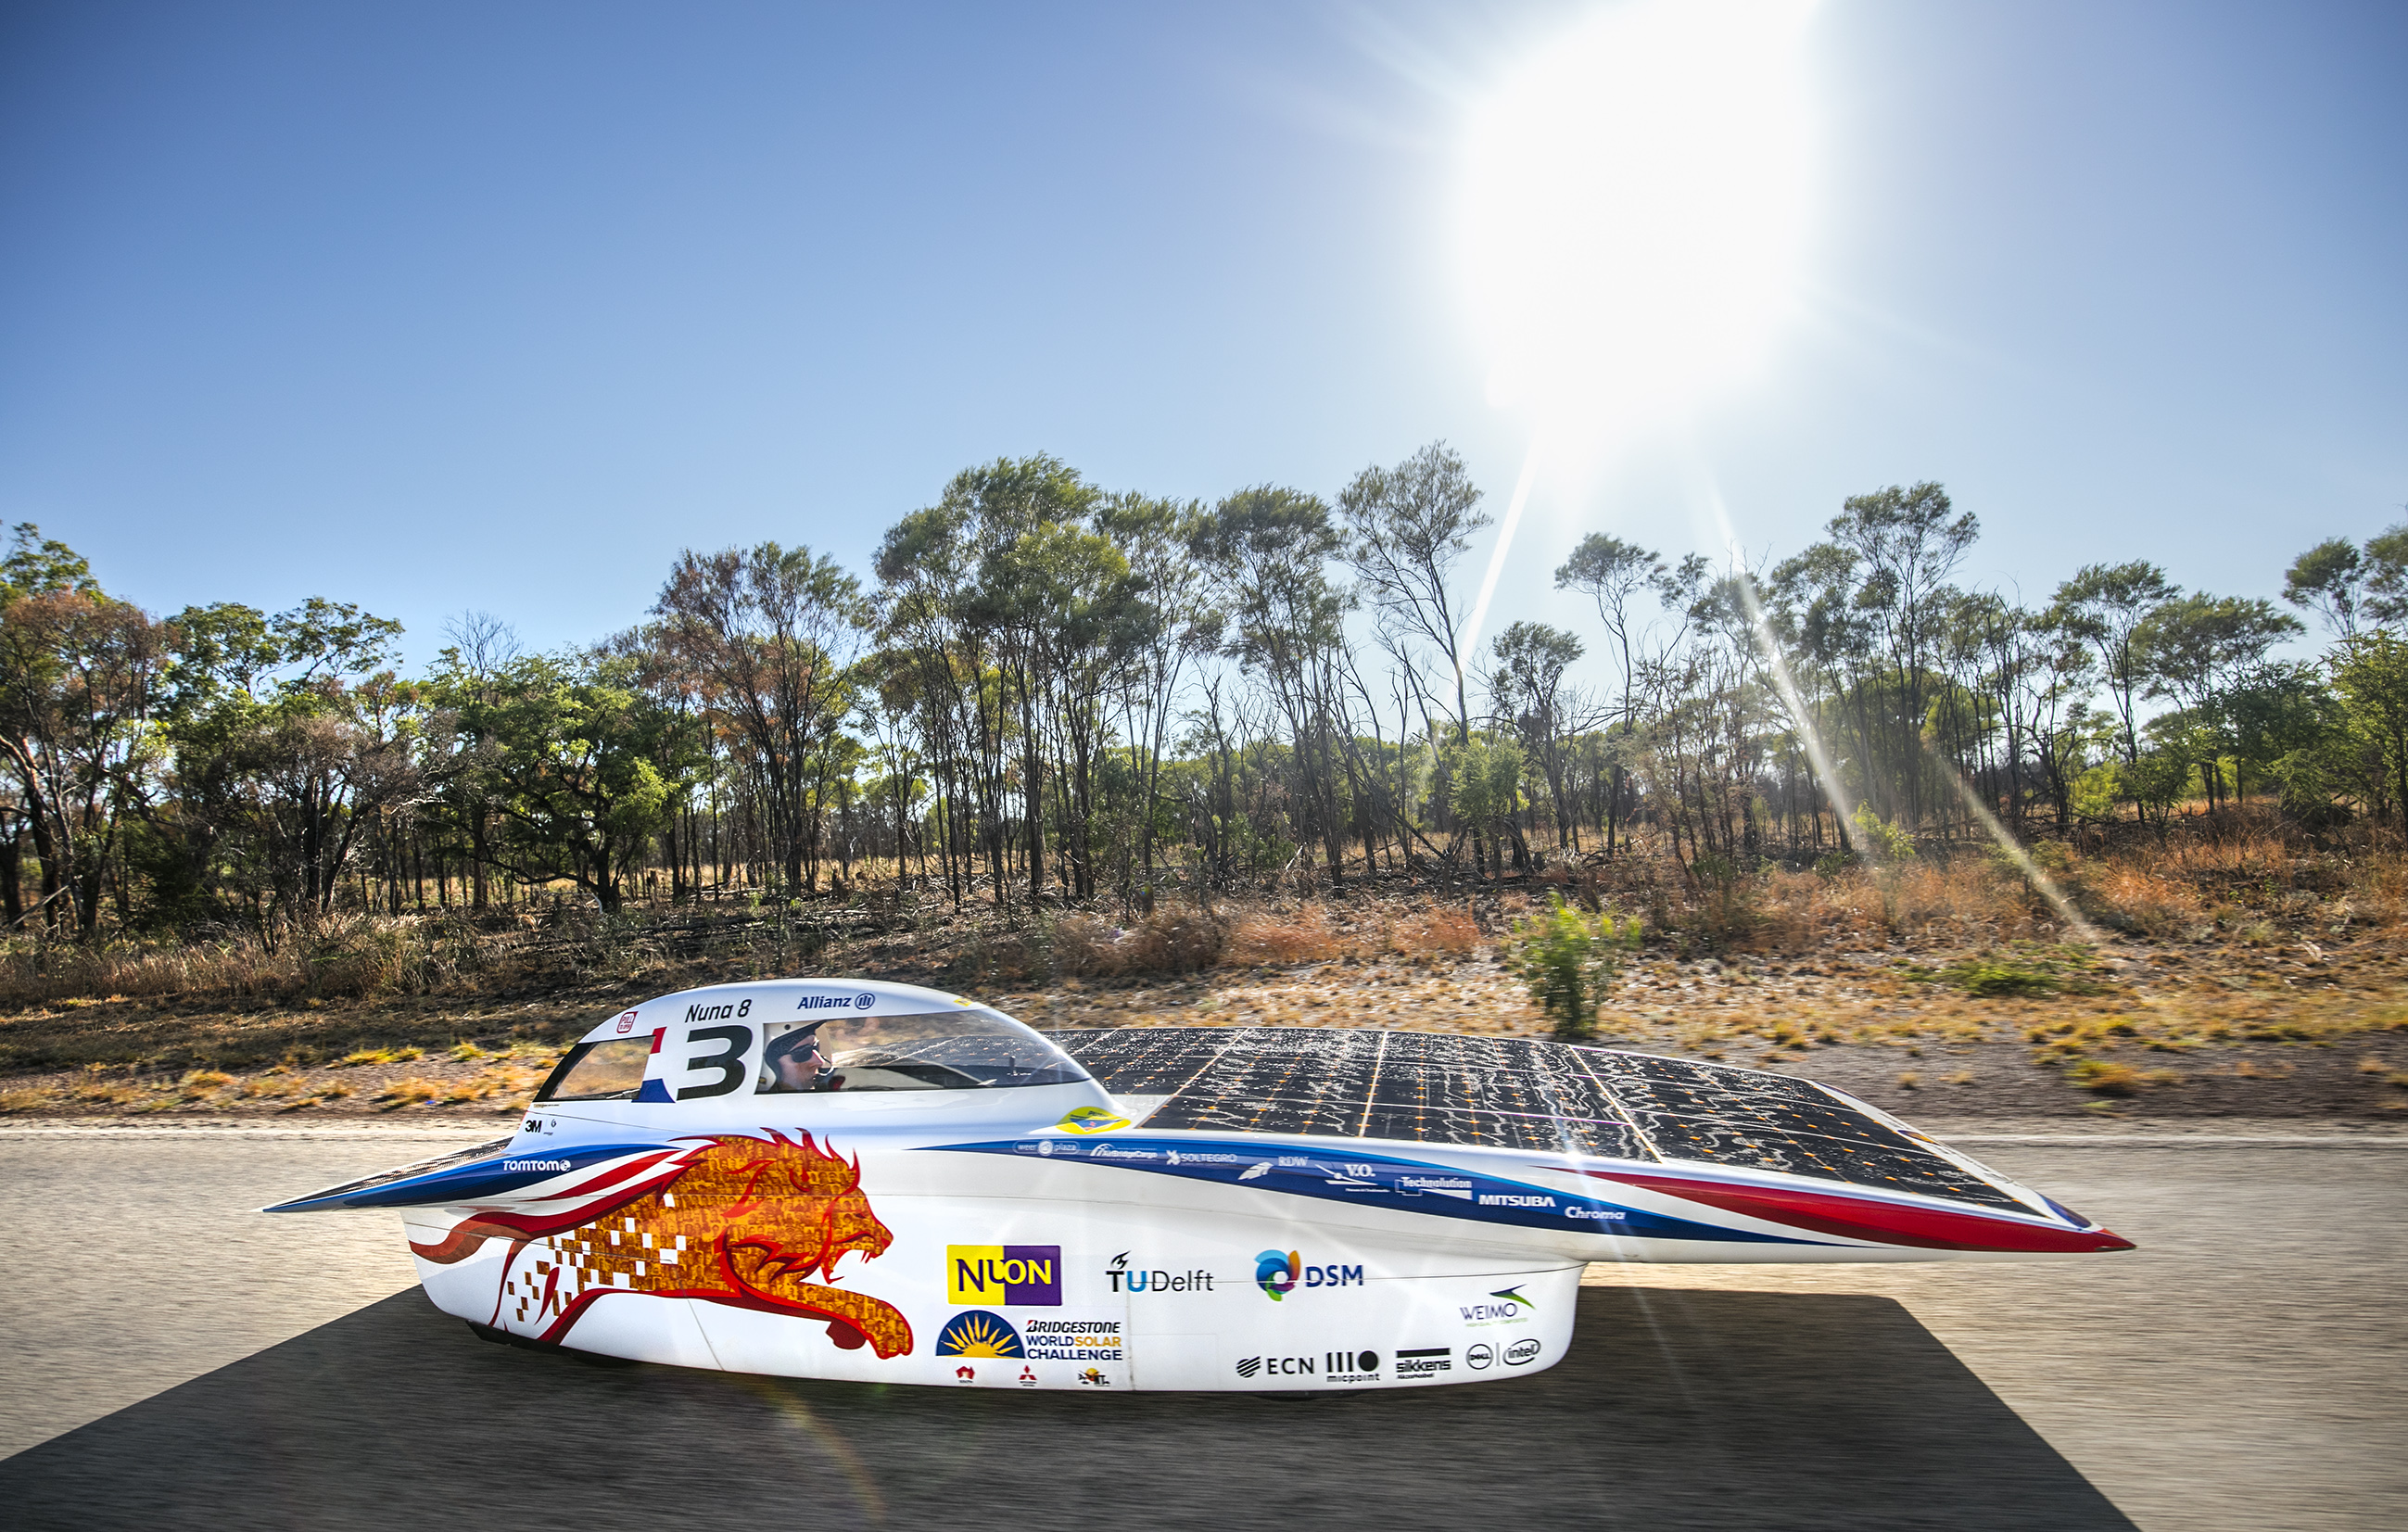
\includegraphics[height=0.25\textheight,width=0.45\textwidth]{textreme_solar_car.jpg}}
  %\caption{Single RVE model.}
  \label{fig:thin-ply-examples}
\end{figure}
\end{frame}

\begin{frame}
\frametitle{\small Spread Tow Technology: Foundations}
\vspace{-0.5cm}
\centering
\begin{figure}
\centering
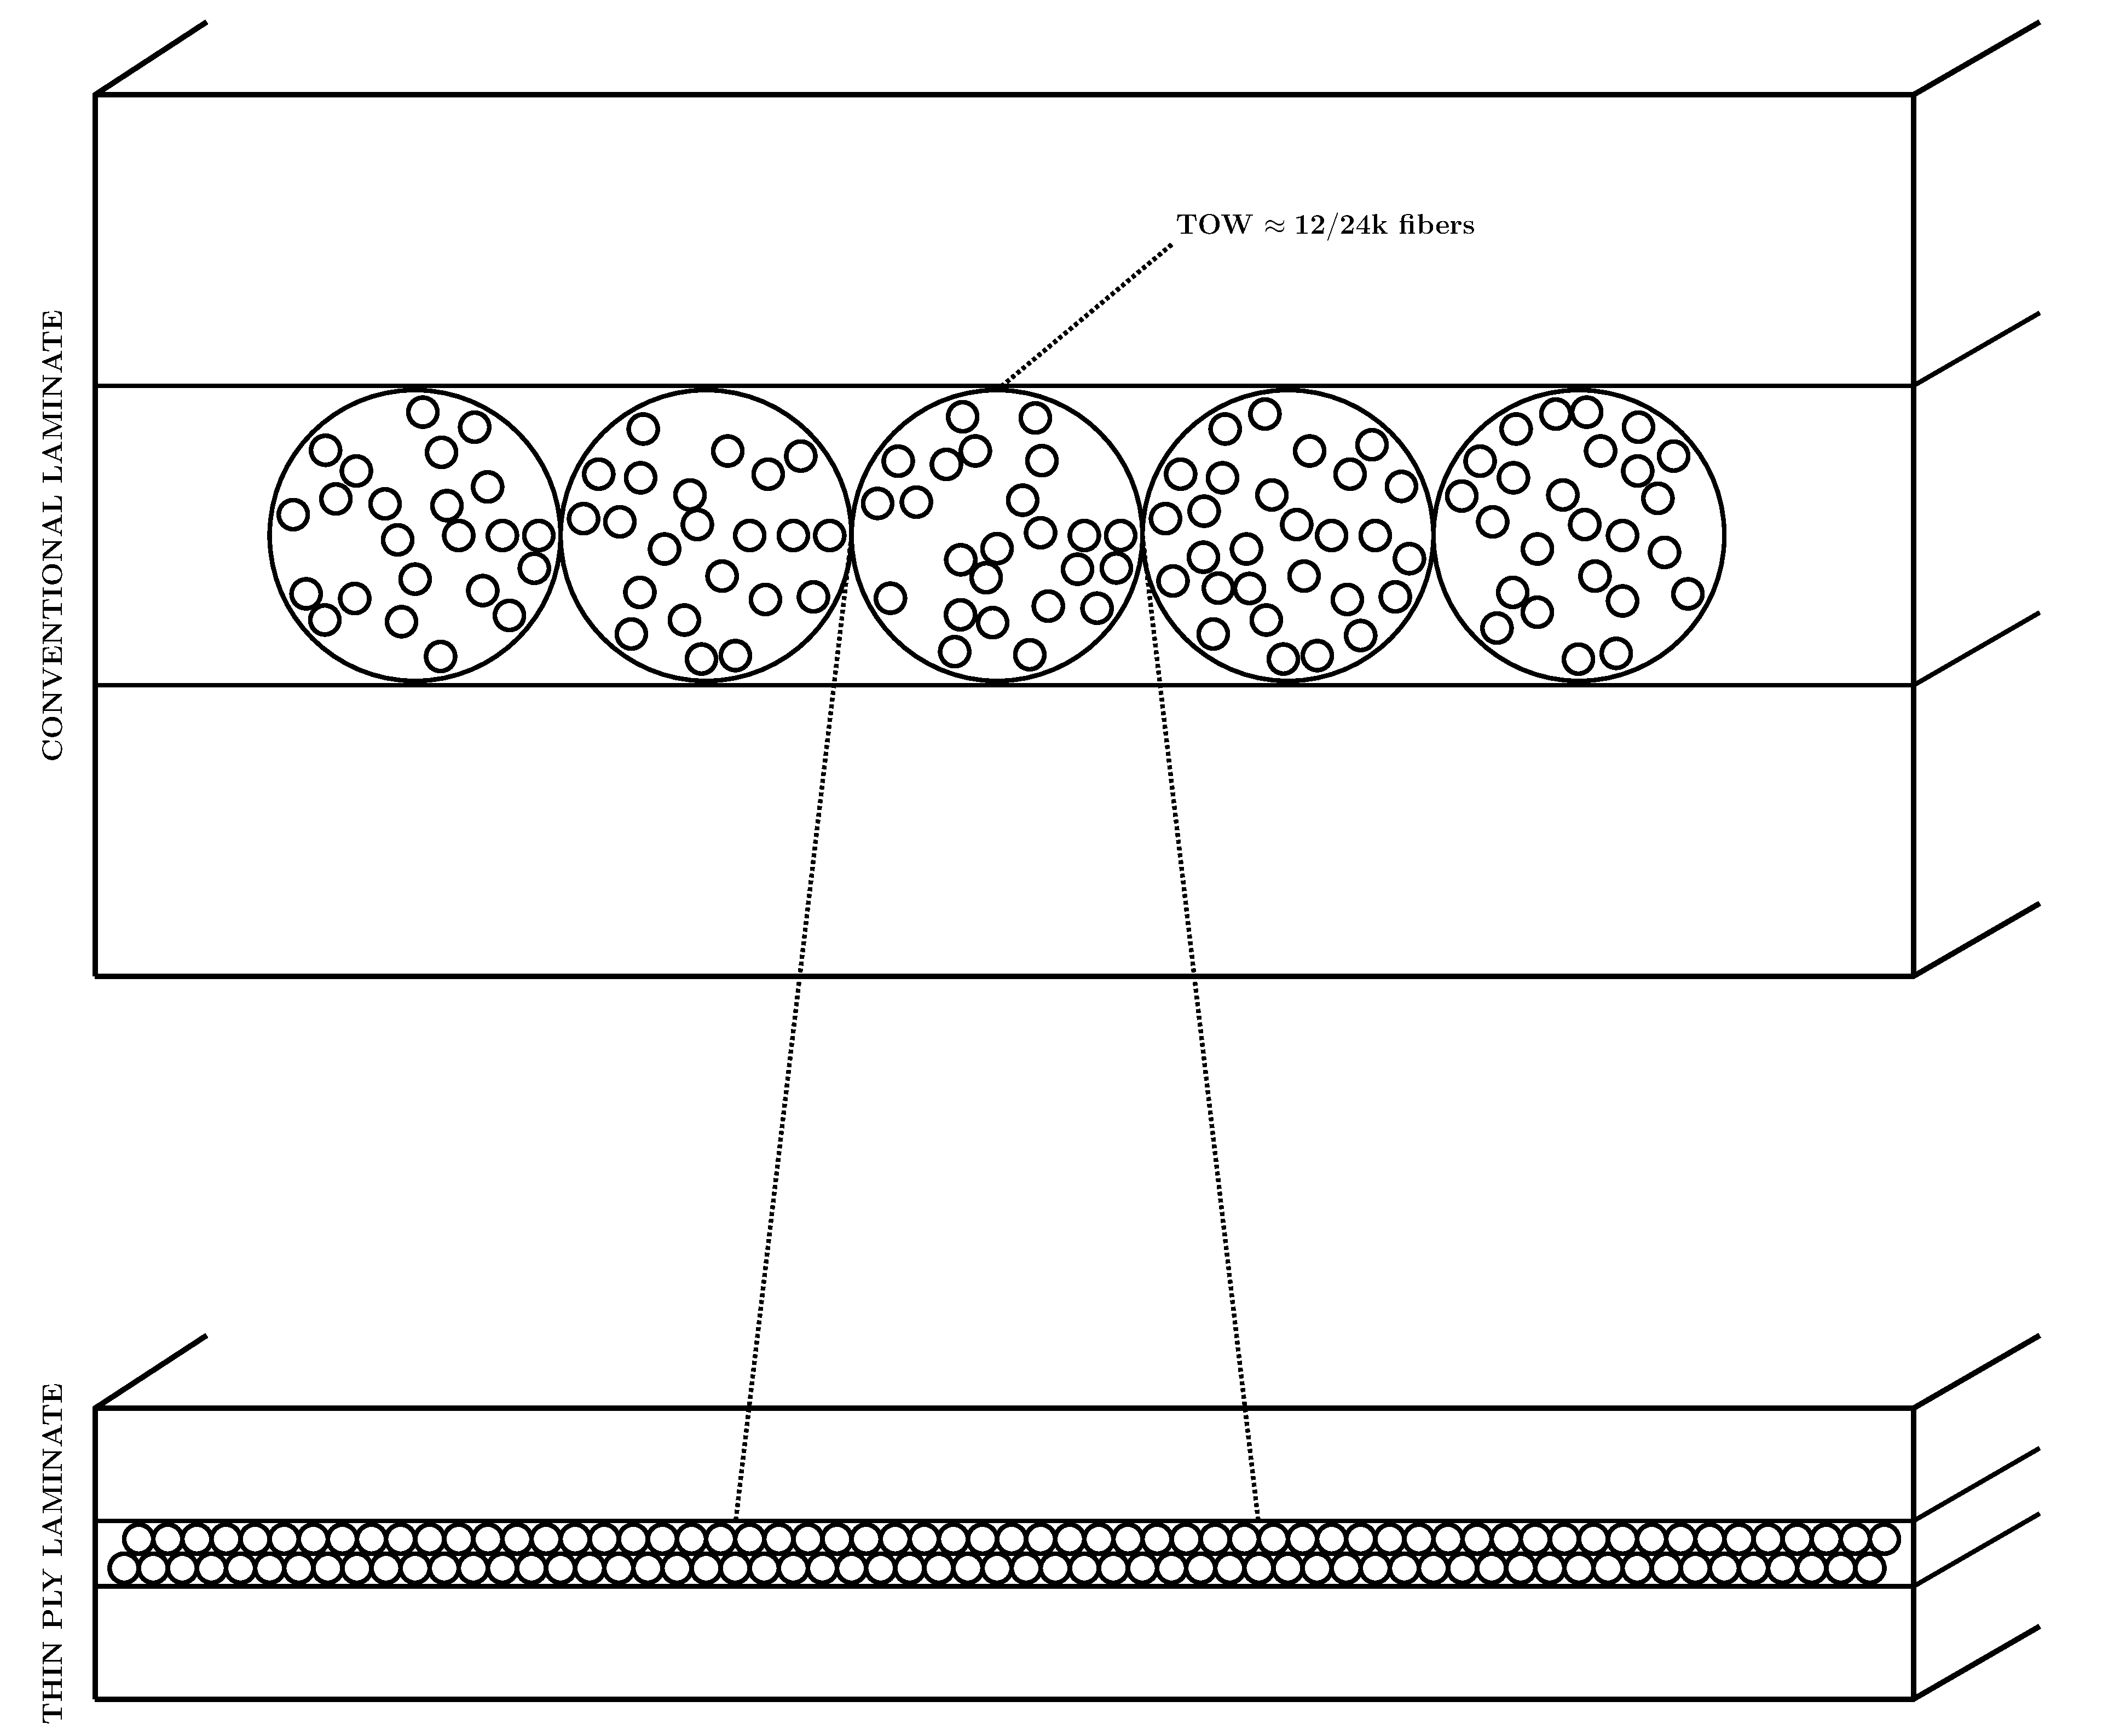
\includegraphics[height=0.85\textheight]{spread-tow-tech.pdf}
%\caption{}
\label{fig:spread-tow-schematic}
\end{figure}
\end{frame}

\subsection{Thin ply effect in transverse cracking}

\begin{frame}
\frametitle{\small Damage Onset and Propagation}
\vspace{-0.75cm}
\centering
\captionsetup[subfigure]{labelfont=footnotesize}
\begin{figure}[!h]
\centering
\subfloat[\scriptsize By Dr. R. Olsson, Swerea, SE.\label{fig:all-cracks}]{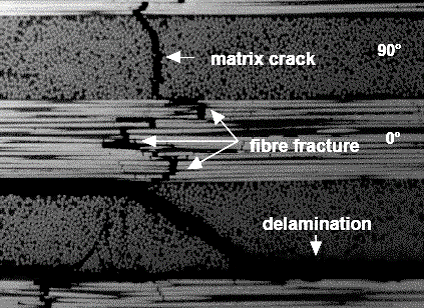
\includegraphics[width=0.46\textwidth]{all-cracks.png}}\quad
\subfloat[\scriptsize By Prof. Dr. E. K. Gamstedt, KTH, SE.\label{fig:transverse-cracks}]{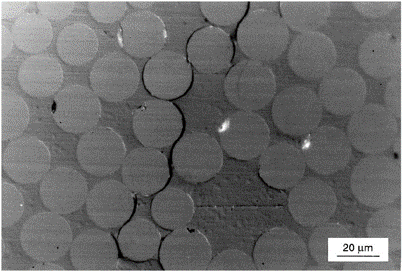
\includegraphics[width=0.5\textwidth]{intralaminar-cracks.png}}
 \caption{For a visual definition of intralaminar transverse cracking.}
  \label{fig:intralaminar-cracks}
\end{figure}
\end{frame}

\begin{frame}
\frametitle{\small The Thin Ply Effect}
\vspace{-0.25cm}
\centering
\begin{figure}[!h]
\centering
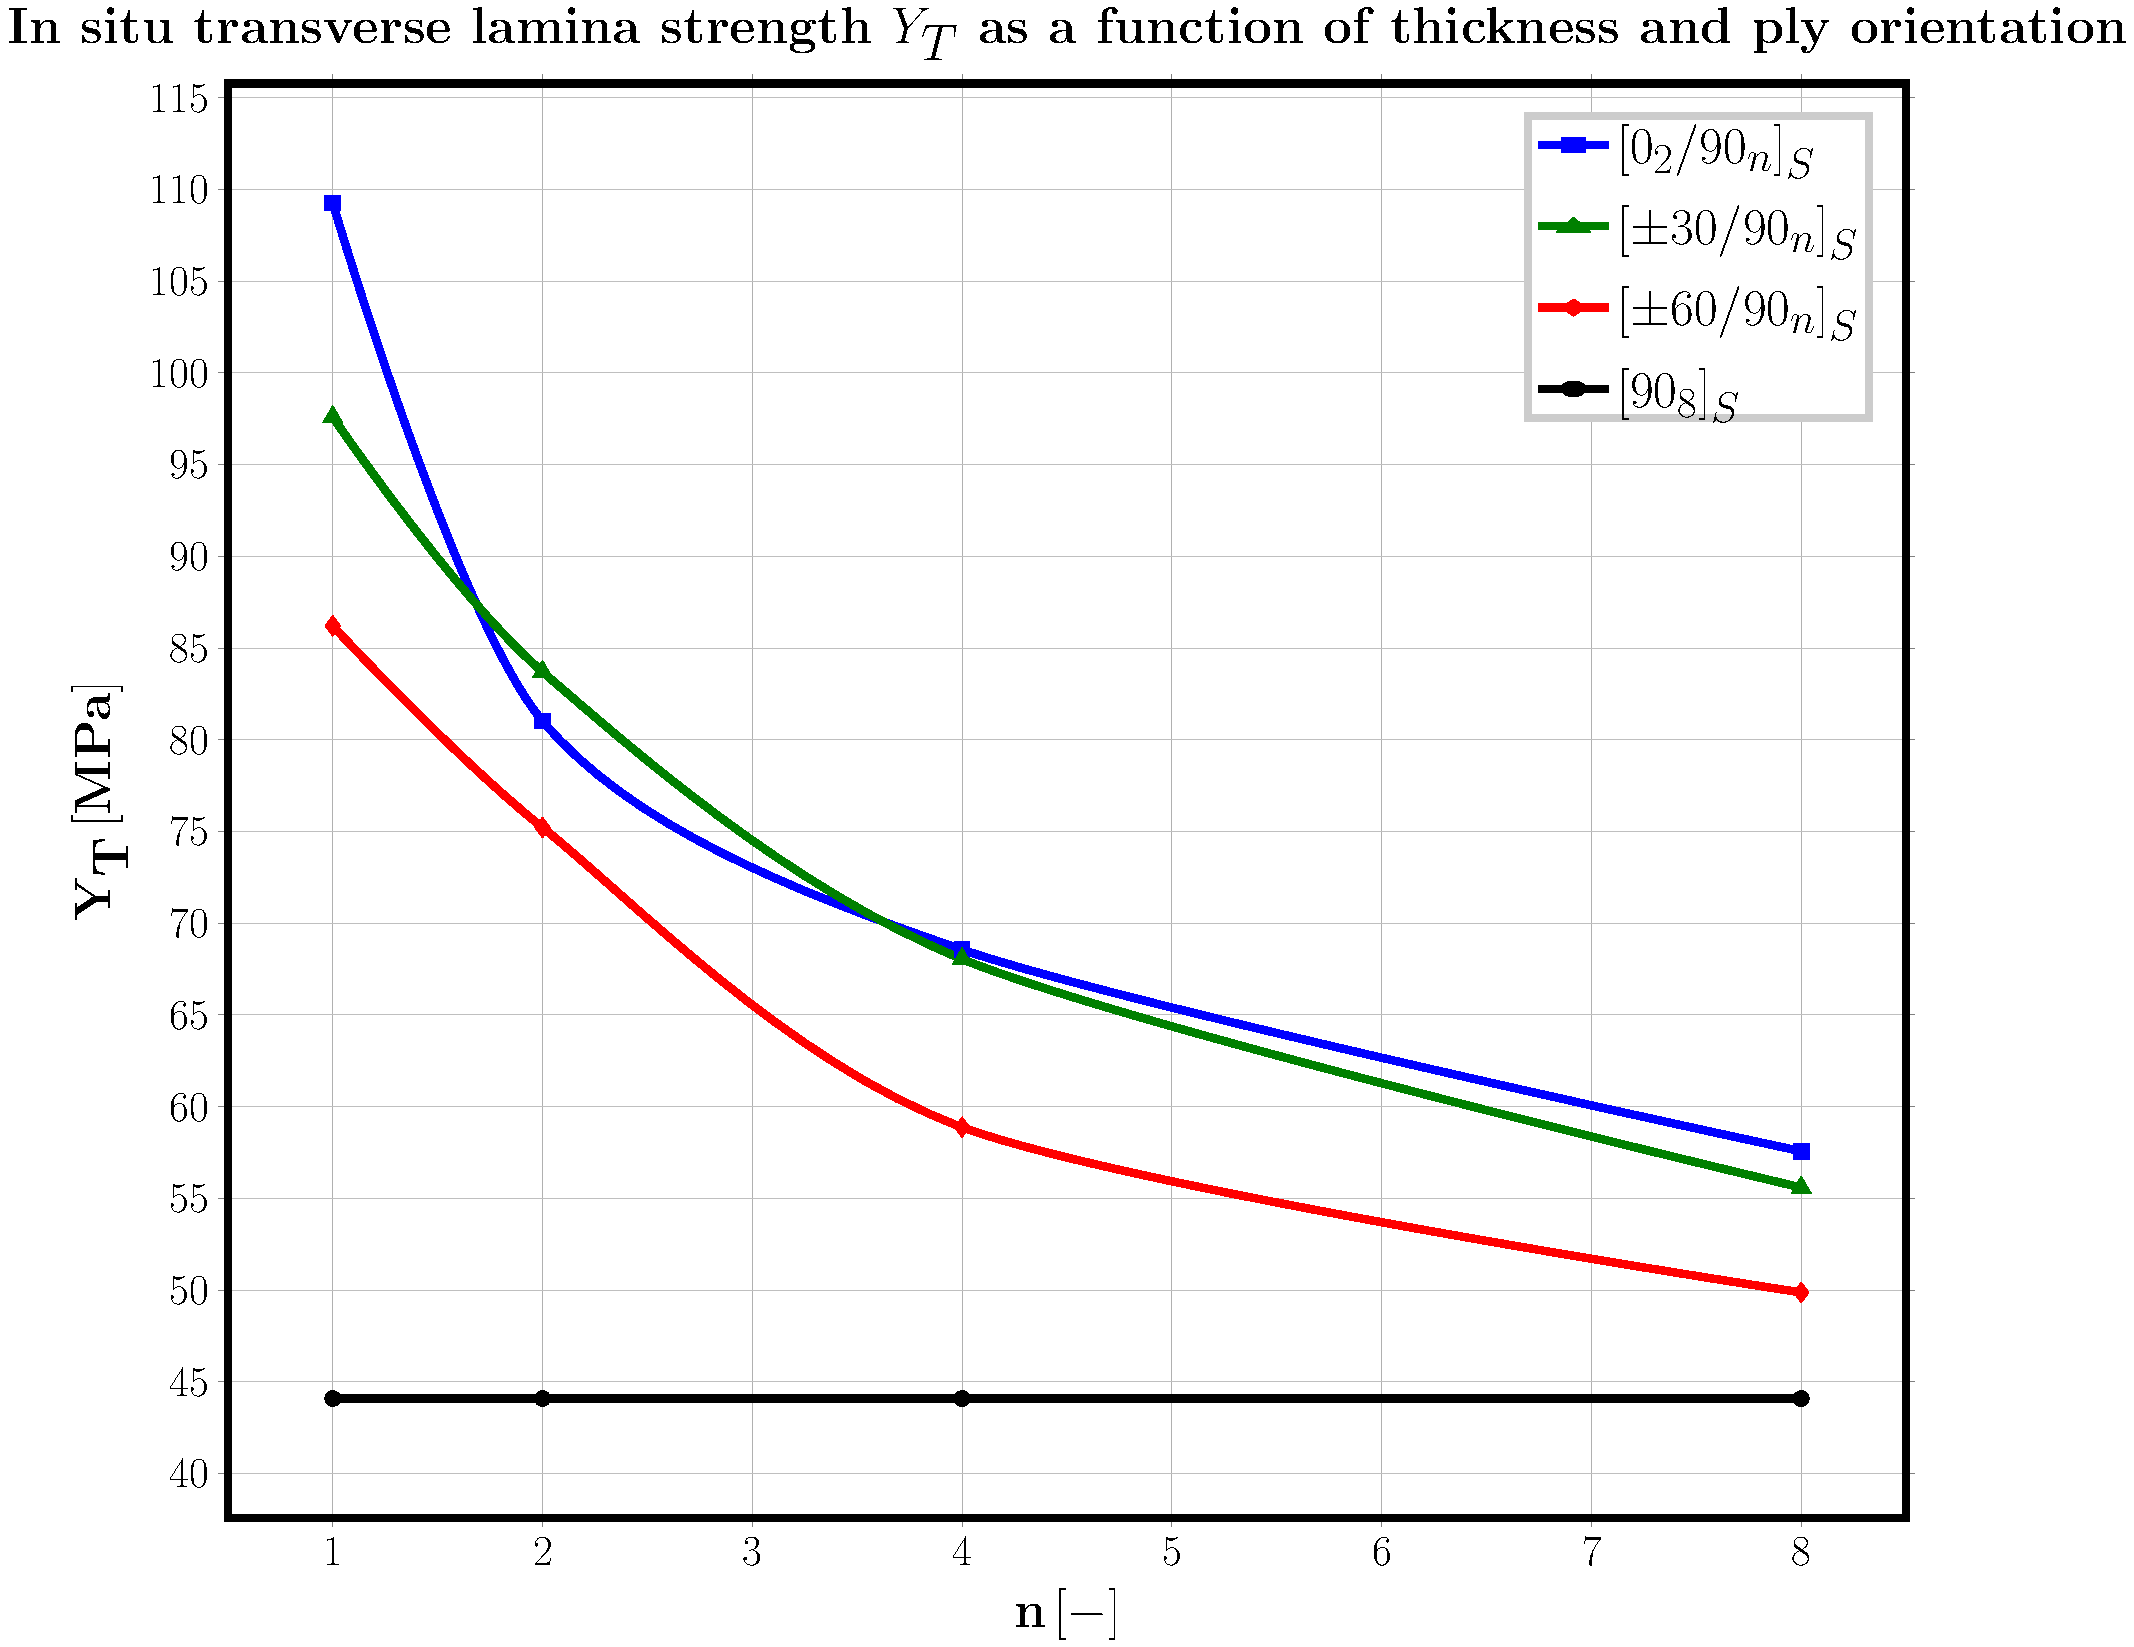
\includegraphics[height=0.75\textheight]{Flaggs-Kural_InSituTransverseStrength.pdf}
\vspace*{-0.3cm}
\caption{\tiny Measurements of in-situ transverse strength from D. L. Flaggs \& M. H. Kural, 1982 [7].}
 \label{fig:in-situ-strength}
\end{figure}
\end{frame}

\subsection[Characterization of Fracture in FRPC]{Characterization of Fracture in FRPC Laminates}

\begin{frame}
%\vspace{-0.5cm}
\frametitle{\small Characterization of the Fracture Process}
\vspace{-0.25cm}
\centering
\scriptsize
\begin{itemize}[label=\ding{212}]
\item Energy Release Rate
\begin{equation*}
G_{m}=G_{m}\left(p_{1},\dots,p_{i},\dots,p_{n}\right)\quad\text{where}\quad G=\frac{\partial W}{\partial A} - \left(\frac{\partial U}{\partial A}+\frac{\partial E_{k}}{\partial A}\right)
\end{equation*}
\item Stress Intensity Factor
\begin{equation*}
K_{m}=K_{m}\left(p_{1},\dots,p_{i},\dots,p_{n}\right)\quad\text{where}\quad \sigma_{m}\sim K_{m}\frac{\alpha}{\left(x-a\right)^{\beta}}\quad\alpha,\beta>0
\end{equation*}
\item J-Integral
\begin{equation*}
J=J\left(p_{1},\dots,p_{i},\dots,p_{n}\right)\quad\text{where}\quad J=\lim_{\varepsilon\to 0}\int_{\Gamma_{\varepsilon}}\left(W\left(\Gamma\right)n_{i}-n_{j}\sigma_{jk}\frac{\partial u_{k}\left(\Gamma,x_{i}\right)}{\partial x_{i}}\right)d\Gamma = G
\end{equation*}
\item Crack Opening \& Shear Displacement
\begin{equation*}
COD=COD\left(p_{1},\dots,p_{i},\dots,p_{n}\right)\quad\text{and}\quad CSD=CSD\left(p_{1},\dots,p_{i},\dots,p_{n}\right)
\end{equation*}
\end{itemize}
\vspace{5pt}
\begin{equation*}
p_{i}\in\left\{\text{geometry},\text{materials},\text{boundary conditions},\text{loading mode},\text{scale}\right\}
\end{equation*}
\begin{equation*}
m\in\left\{I,II,III,I/II,I/III,II/III\right\}
\end{equation*}
\end{frame}


\begin{frame}
\frametitle{\small Evaluation of Fracture Parameters}
\vspace{-0.4cm}
\centering
\tiny
\begin{columns}
\begin{column}{0.5\textwidth}
\begin{itemize}[label=\ding{212}]
\item \bf{Analytical}
\begin{list}{\Large\textcolor{green}{$\mathbf{\checkmark}$}}{}
\item Closed form
\item Every material scale can be studied
\end{list}
\begin{list}{\Huge\textcolor{red}{$\mathbf{\times}$}}{}
\item Particular configurations, often infinite in size
\item Complex geometries cannot be studied
\end{list}
\end{itemize}
\end{column}
\begin{column}{0.5\textwidth}
\begin{itemize}[label=\ding{212}]
\item \bf{Numerical}
\begin{list}{\Large\textcolor{green}{$\mathbf{\checkmark}$}}{}
\item Complex geometries can be studied
\item Every material scale can be studied
\end{list}
\begin{list}{\Huge\textcolor{red}{$\mathbf{\times}$}}{}
\item Discretization
\item Finite domains
\end{list}
\end{itemize}
\end{column}
\end{columns}
\vspace*{0.5cm}
\begin{columns}
\begin{column}{0.3\textwidth}
\end{column}
\begin{column}{0.5\textwidth}
\begin{itemize}[label=\ding{212}]
\item \bf{Experimental}
\begin{list}{\Large\textcolor{green}{$\mathbf{\checkmark}$}}{}
\item Complex geometries can be studied
\end{list}
\begin{list}{\Huge\textcolor{red}{$\mathbf{\times}$}}{}
\item Not every material scale is accessible
\end{list}
\end{itemize}
\end{column}
\begin{column}{0.2\textwidth}
\end{column}
\end{columns}

\end{frame}

\begin{frame}
\frametitle{\small Numerical Estimation of Energy Release Rates}
\vspace{-0.4cm}
\centering
\scriptsize
\begin{columns}
\begin{column}{0.5\textwidth}
\centering
\vspace*{-1.4cm}
\begin{itemize}[label=\ding{212}]
\item Virtual Crack Closure Technique (VCCT)
\begin{figure}
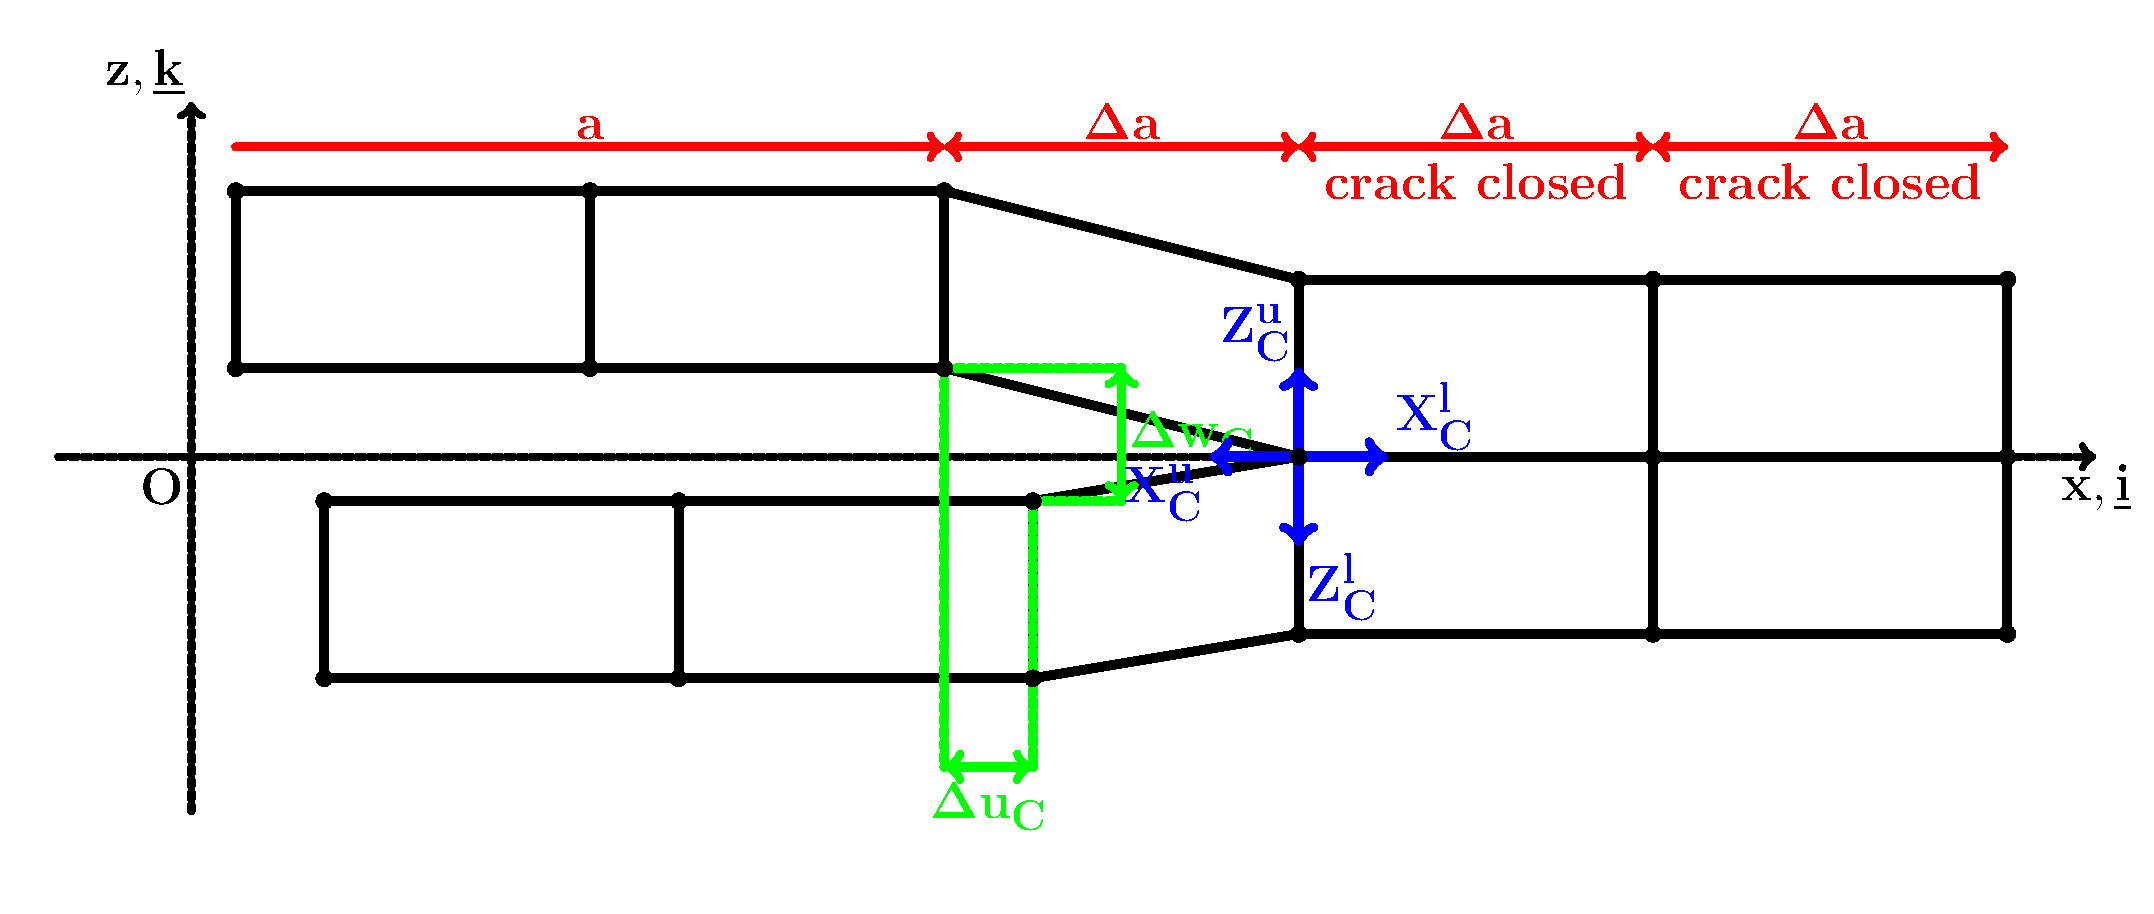
\includegraphics[width=\columnwidth]{VCCT.pdf}
 % \caption{VCCT}
  \label{fig:vcct}
\end{figure}

\begin{equation*}
G_{I}=\frac{Z_{C}\Delta w_{C}}{2B\Delta a}\quad G_{II}=\frac{X_{C}\Delta u_{C}}{2B\Delta a}
\end{equation*}

Krueger, 2004
\end{itemize}
\end{column}
\begin{column}{0.5\textwidth}
\centering
\begin{itemize}[label=\ding{212}]
\item J-Integral

\begin{figure}
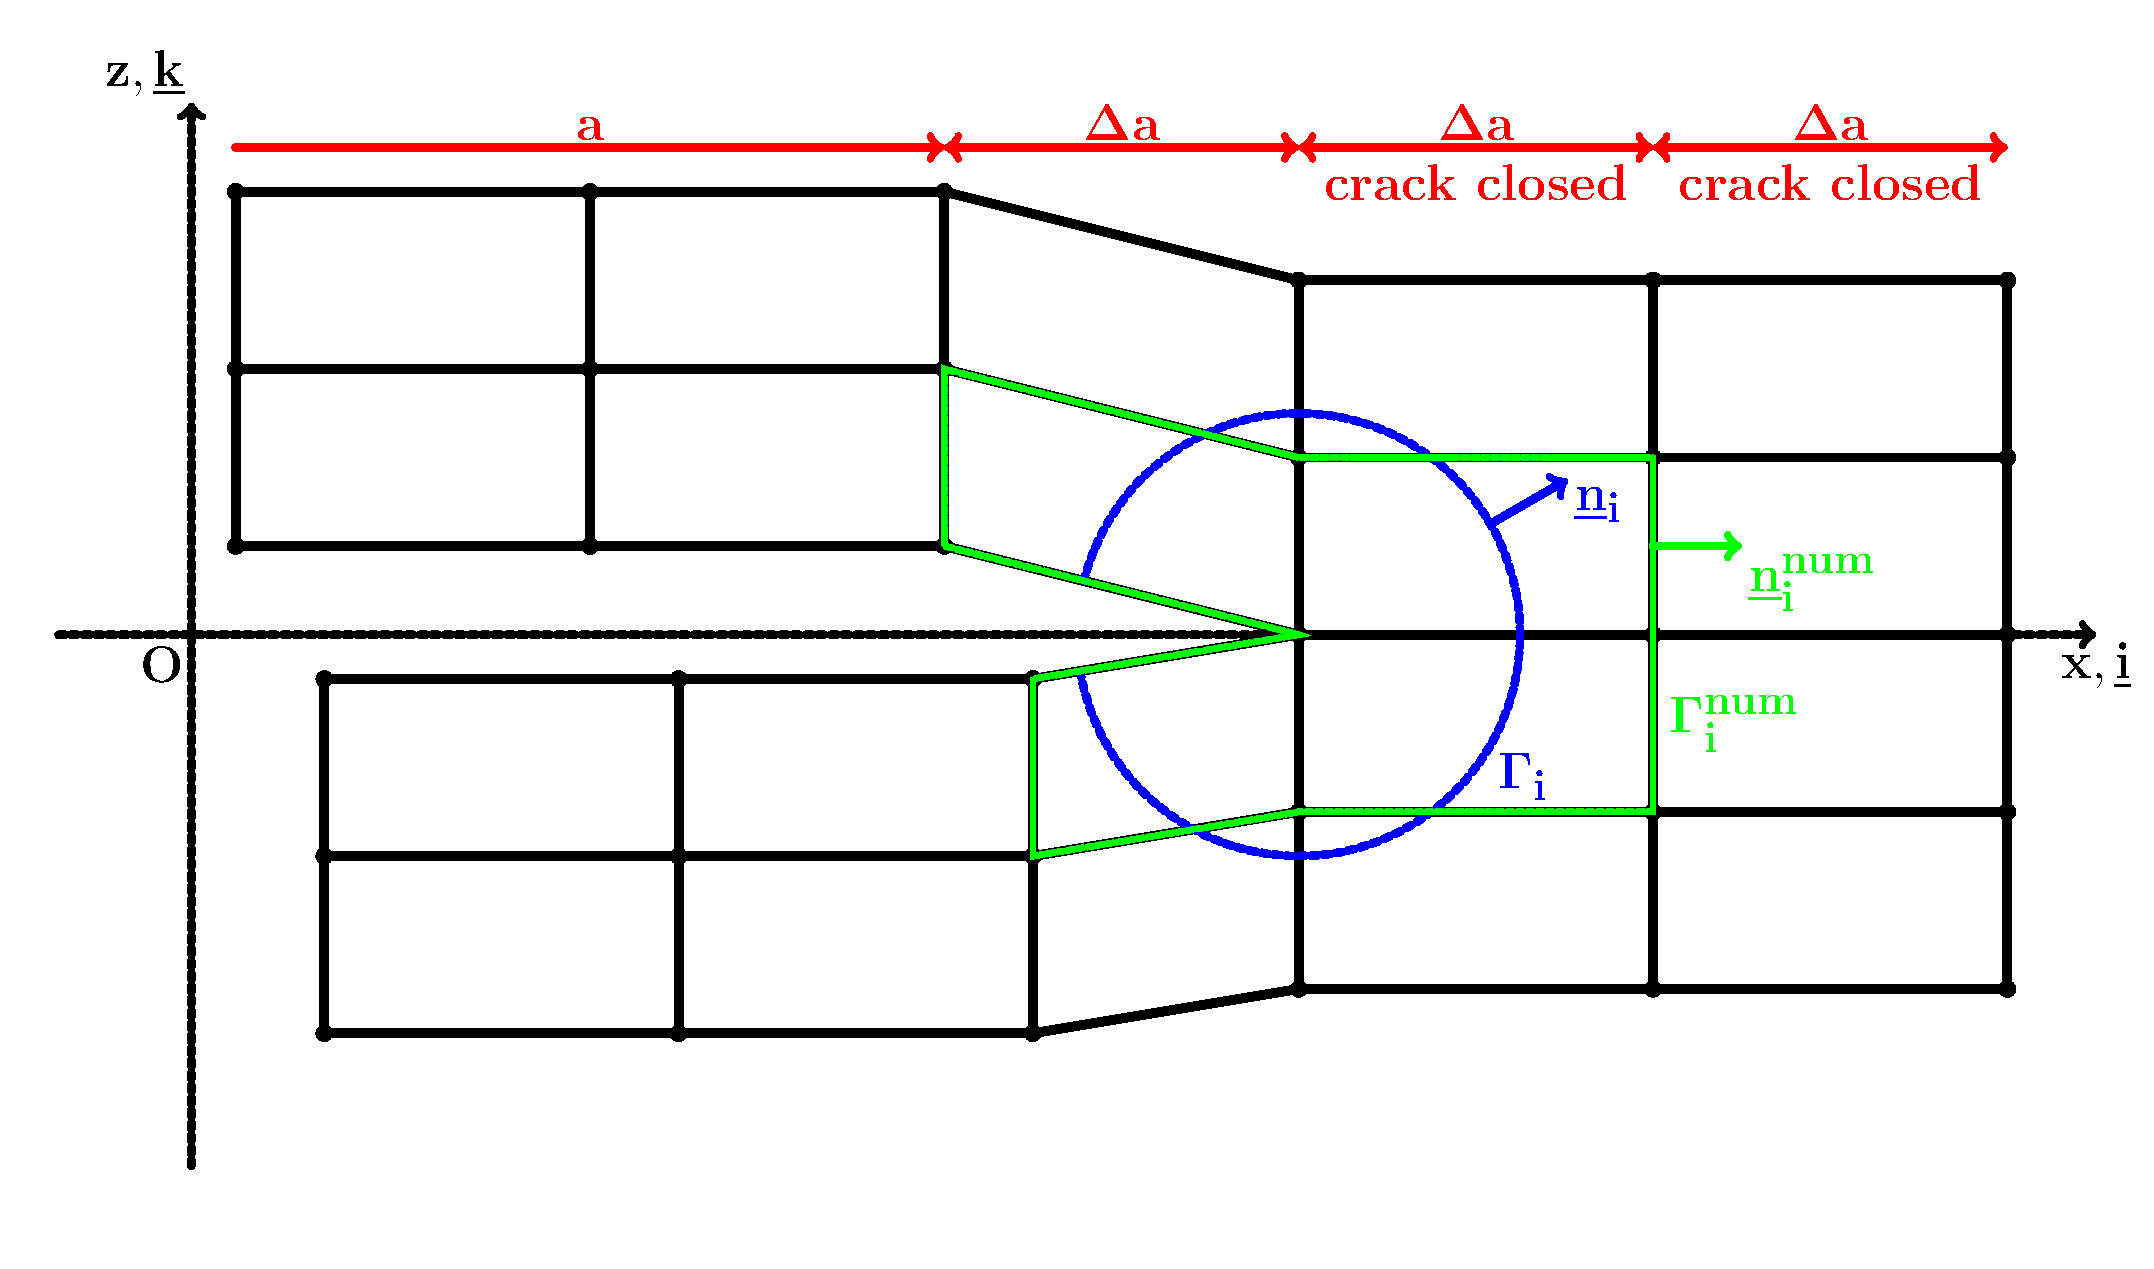
\includegraphics[width=\columnwidth]{J-integral.pdf}
 % \caption{Angular discretization at fiber/matrix interface.}
  \label{fig:jintegral}
\end{figure}

\begin{equation*}
J_{i}=\lim_{\varepsilon\to 0}\int_{\Gamma_{\varepsilon}}\left(W\left(\Gamma\right)n_{i}-n_{j}\sigma_{jk}\frac{\partial u_{k}\left(\Gamma,x_{i}\right)}{\partial x_{i}}\right)d\Gamma
\end{equation*}

Rice, 1968
\end{itemize}
\end{column}
\end{columns}
\end{frame}

\section[The Fiber-Matrix Interface Problem in FRPC]{The Fiber-Matrix Interface Problem in Fiber Reinforced Polymer Laminates}

\subsection{Multi-Scale Decomposition}

\begin{frame}
\frametitle{\small Multi-scale Decomposition of Fiber Reinforced Polymer Laminates}
\vspace{-1cm}
\centering
\begin{figure}
\centering
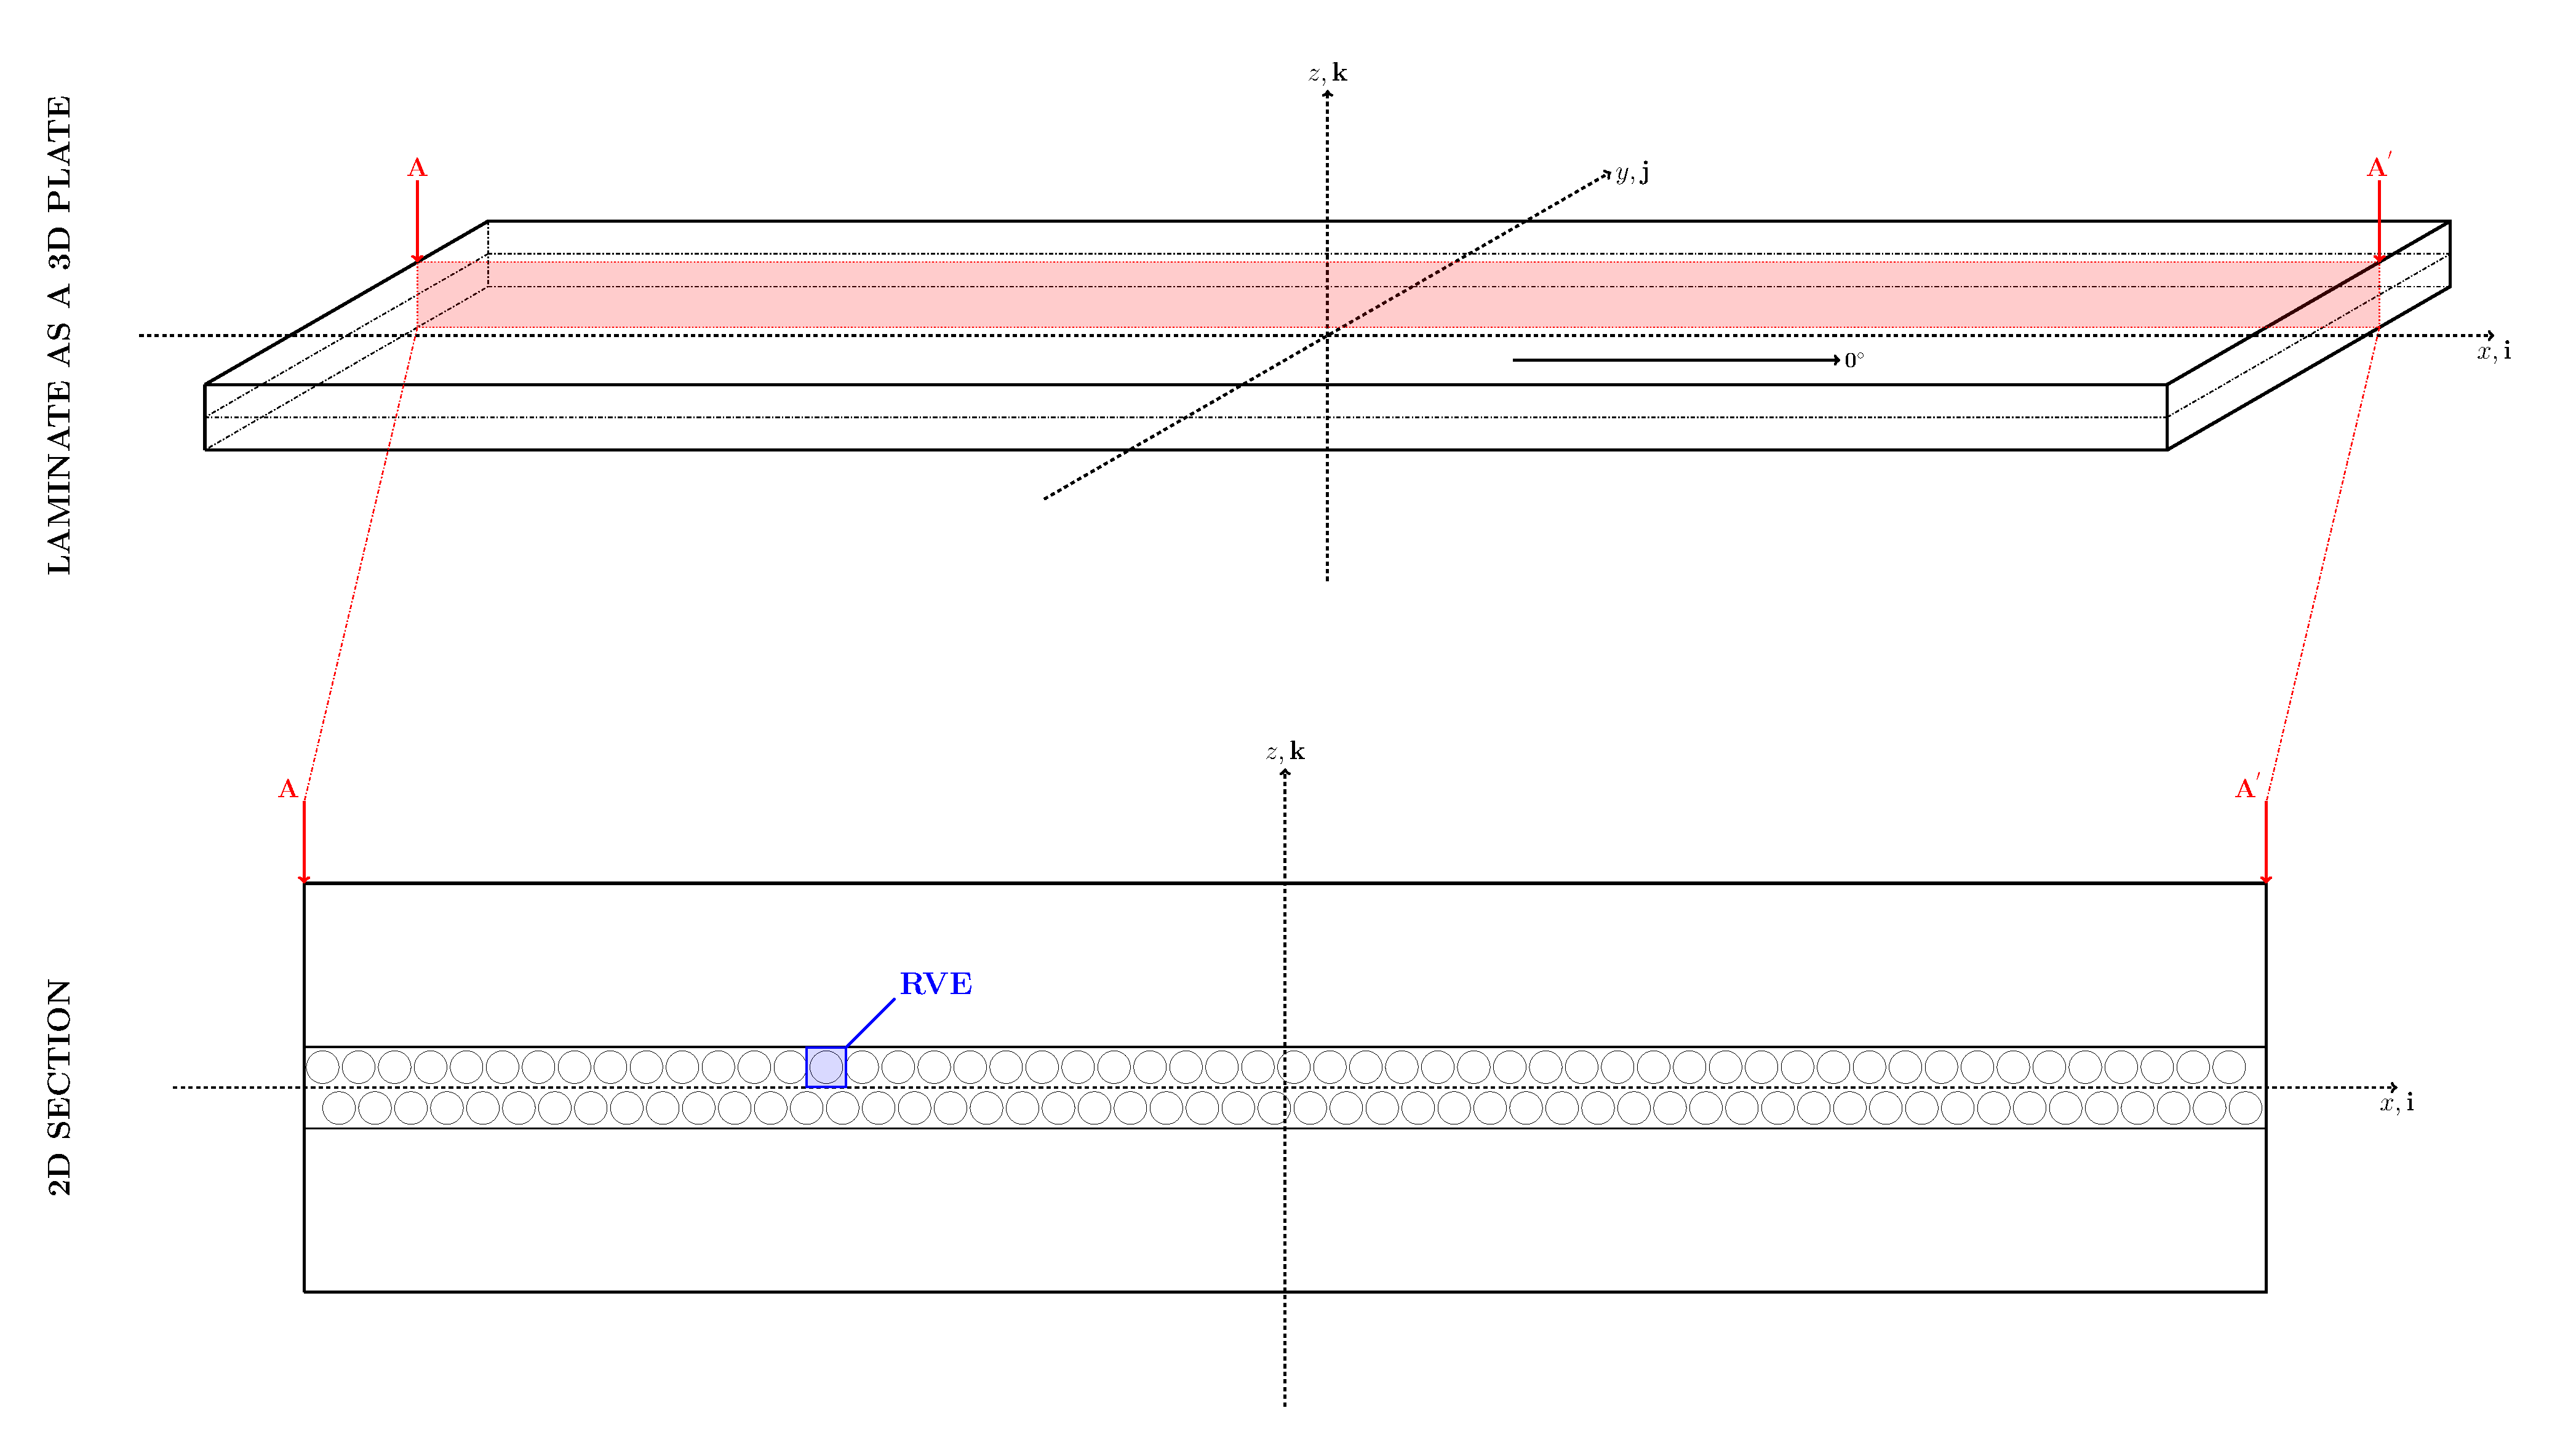
\includegraphics[height=0.8\textheight]{laminate-section.pdf}
%\caption{}
\label{fig:spread-tow-schematic}
\end{figure}
\end{frame}

\subsection{The Fiber-Matrix Interface Crack Problem}

\begin{frame}
\frametitle{\small The Fiber-Matrix Interface Crack Problem: Statement}
\vspace{-0.5cm}
\centering
\begin{columns}
\begin{column}{0.7\textwidth}
\begin{figure}
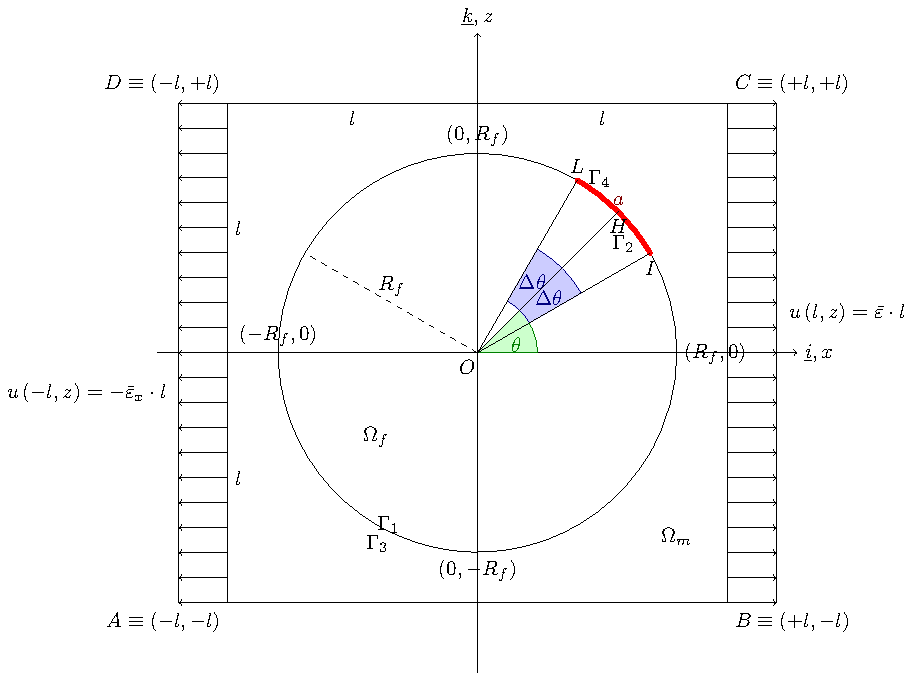
\includegraphics[width=\columnwidth]{FEMfiberMatrixInterfaceProblem.pdf}
 % \caption{Angular discretization at fiber/matrix interface.}
  \label{fig:jintegral}
\end{figure}
\end{column}
\begin{column}{0.3\textwidth}
\scriptsize
\begin{itemize}[label=\ding{212}]
\item 2D space
\item Linear elastic homogeneous isotropic materials
\item Mismatching elastic properties
\item Plane state (strain or stress)
%\item Displacement-controlled
\item Dirichlet-type BC
\item Linear Fracture Mechanics
\item Contact interaction
\item Applied uniaxial traction
%\item Bi-linear quadrilateral elements
\end{itemize}
\begin{itemize}[label=?]
\item SIF, ERR, mode ratio, stress and displacement distribution at the interface
\end{itemize}
\end{column}
\end{columns}
\end{frame}

\begin{frame}
\frametitle{\small The Fiber-Matrix Interface Crack Problem: Solution}
\vspace{-0.5cm}
\centering
\footnotesize
\begin{table}
\begin{tabularx}{\columnwidth}{p{0.2\textwidth}Xp{0.3\textwidth}XX}
{\tiny \bf{Method}}&{\tiny \bf{Domain}}&{\tiny \bf{Natural Variable}}&{\tiny \bf{Conjugate Variable}}&{\tiny \bf{Dirichlet BC}}\\
\toprule
{\tiny Analytical (complex) functions}&{\tiny 2D, continuous, infinite}&{\tiny Airy stress potential \& stress}&{\tiny Displacement \& strain}&{\tiny In stress}\\[10pt]
\cline{2-5}\\[-10pt]
&\multicolumn{4}{p{0.7\textwidth}}{\tiny M. Toya (1975), A Crack Along the Interface of a Circular Inclusion Embedded in an Infinite Solid [10].}\\
\bottomrule
{\tiny Boundary Element Method (BEM)}&{\tiny 1D, discrete, finite}&{\tiny Stress, by using Green's potentials or Betti's influence functions}&{\tiny Displacement \& strain}&{\tiny In stress}\\[10pt]
\cline{2-5}\\[-10pt]
&\multicolumn{4}{p{0.7\textwidth}}{\tiny F. Par\'is et al. (1996), The fiber-matrix interface crack - A numerical analysis using Boundary Elements [11].}\\
\bottomrule
{\tiny Finite Element Method (FEM)}&{\tiny 2D, discrete, finite}&{\tiny Displacement}&{\tiny Stress}&{\tiny In displacement}\\[10pt]
\bottomrule
\end{tabularx}
\end{table}
\end{frame}

\section[Analysis of the Infinite RVE]{Analysis of the Infinite Reference Volume Element (RVE)}

\subsection{The Finite Element Model}

\begin{frame}
\frametitle{\small The Finite Element Model}
\vspace{-0.5cm}
\centering
\begin{columns}
\begin{column}{0.6\textwidth}
\begin{figure}
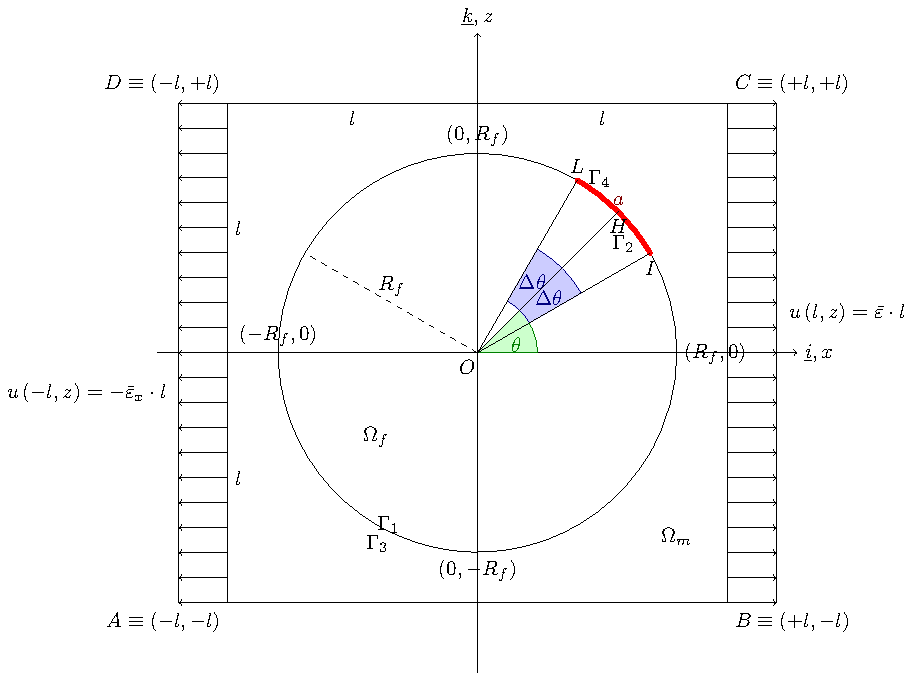
\includegraphics[width=\columnwidth]{FEMfiberMatrixInterfaceProblem.pdf}
 % \caption{Angular discretization at fiber/matrix interface.}
  \label{fig:jintegral}
\end{figure}
\end{column}
\begin{column}{0.4\textwidth}
\tiny
\begin{itemize}[label=\ding{212}]
\item $\theta\left[^{\circ}\right]=0$, angular position of debond's center\\[5pt]
\item $2\Delta\theta\left[^{\circ}\right]$, debond's angular size\\[5pt]
\item $\delta\left[^{\circ}\right]$, angle subtended by an element at the fiber/matrix interface\\[5pt]
\item $VF_{f}\left[-\right]$, fiber volume fraction\\[5pt]
\item $2L\left[\mu m\right]$, RVE's side length\\[5pt]
\item $R_{F}\left[\mu m\right]$, fiber radius\\[5pt]
\item $\frac{L}{R_{f}}=\frac{1}{2}\sqrt{\frac{\pi}{VF_{f}}}\left[-\right]$, RVE's aspect ratio\\[5pt]
\item $\sigma_{0}\left[MPa\right]=\frac{E_{m}}{1-\nu_{m}^{2}}\varepsilon_{xx}$, reaction stress of undamaged infinite RVE\\[5pt]
\item $G_{0}\left[\frac{J}{m^{2}}\right]=\pi R_{f}\sigma_{R}^{2}\frac{1+\left(3-4 nu_{m}\right)}{8 G_{m}}$, normalization $G$ following Toya [10] and Par\'is [11]\\[5pt]
\item Small displacement formulation
\end{itemize}
\end{column}
\end{columns}
\end{frame}

\subsection{Reaction Stress at the Boundary}

\begin{frame}
\frametitle{\small Reaction Stress at the Boundary}
\vspace{-0.5cm}
\centering
\begin{columns}
\begin{column}{0.55\textwidth}
\begin{figure}
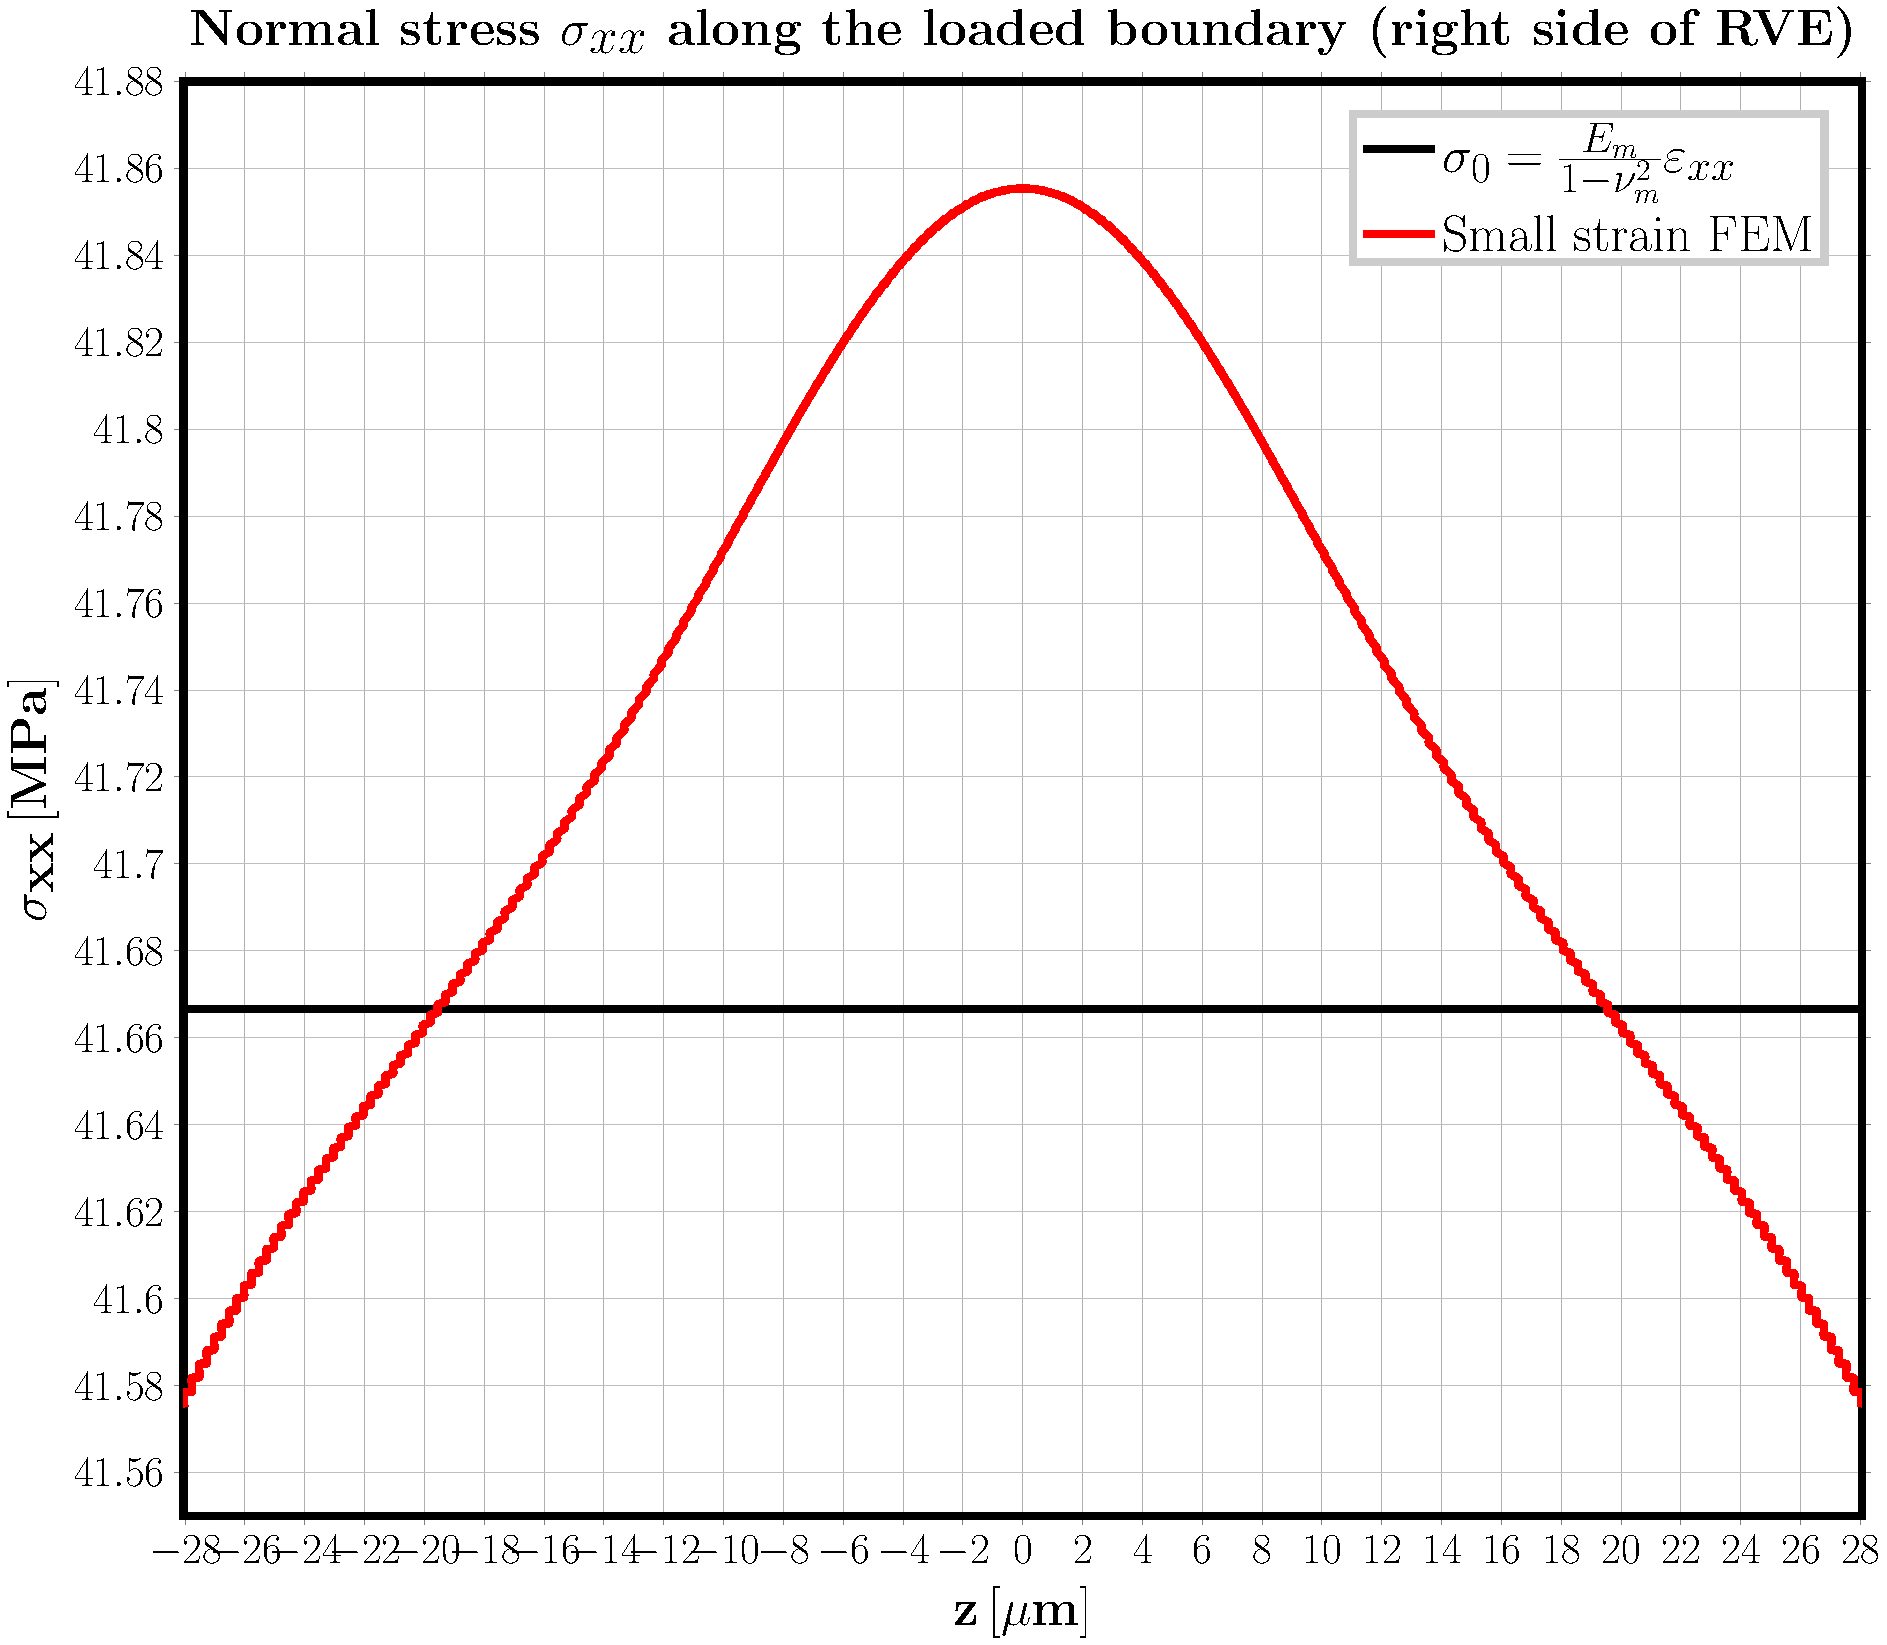
\includegraphics[width=\columnwidth]{2017-06-23_AbqRunSummary_SingleFiberEqRfFiniteStrain_sigmaatboundary_Summary.pdf}
\caption{\scriptsize $VF_{f}=0.001$, $\frac{L}{R_{f}}\sim 28$, $\delta = 0.4^{\circ}$, $\frac{\sigma_{max}-\sigma_{mean}}{\sigma_{mean}}=0.34\%$}
%  \label{fig:jintegral}
\end{figure}
\end{column}
\begin{column}{0.55\textwidth}
\begin{figure}
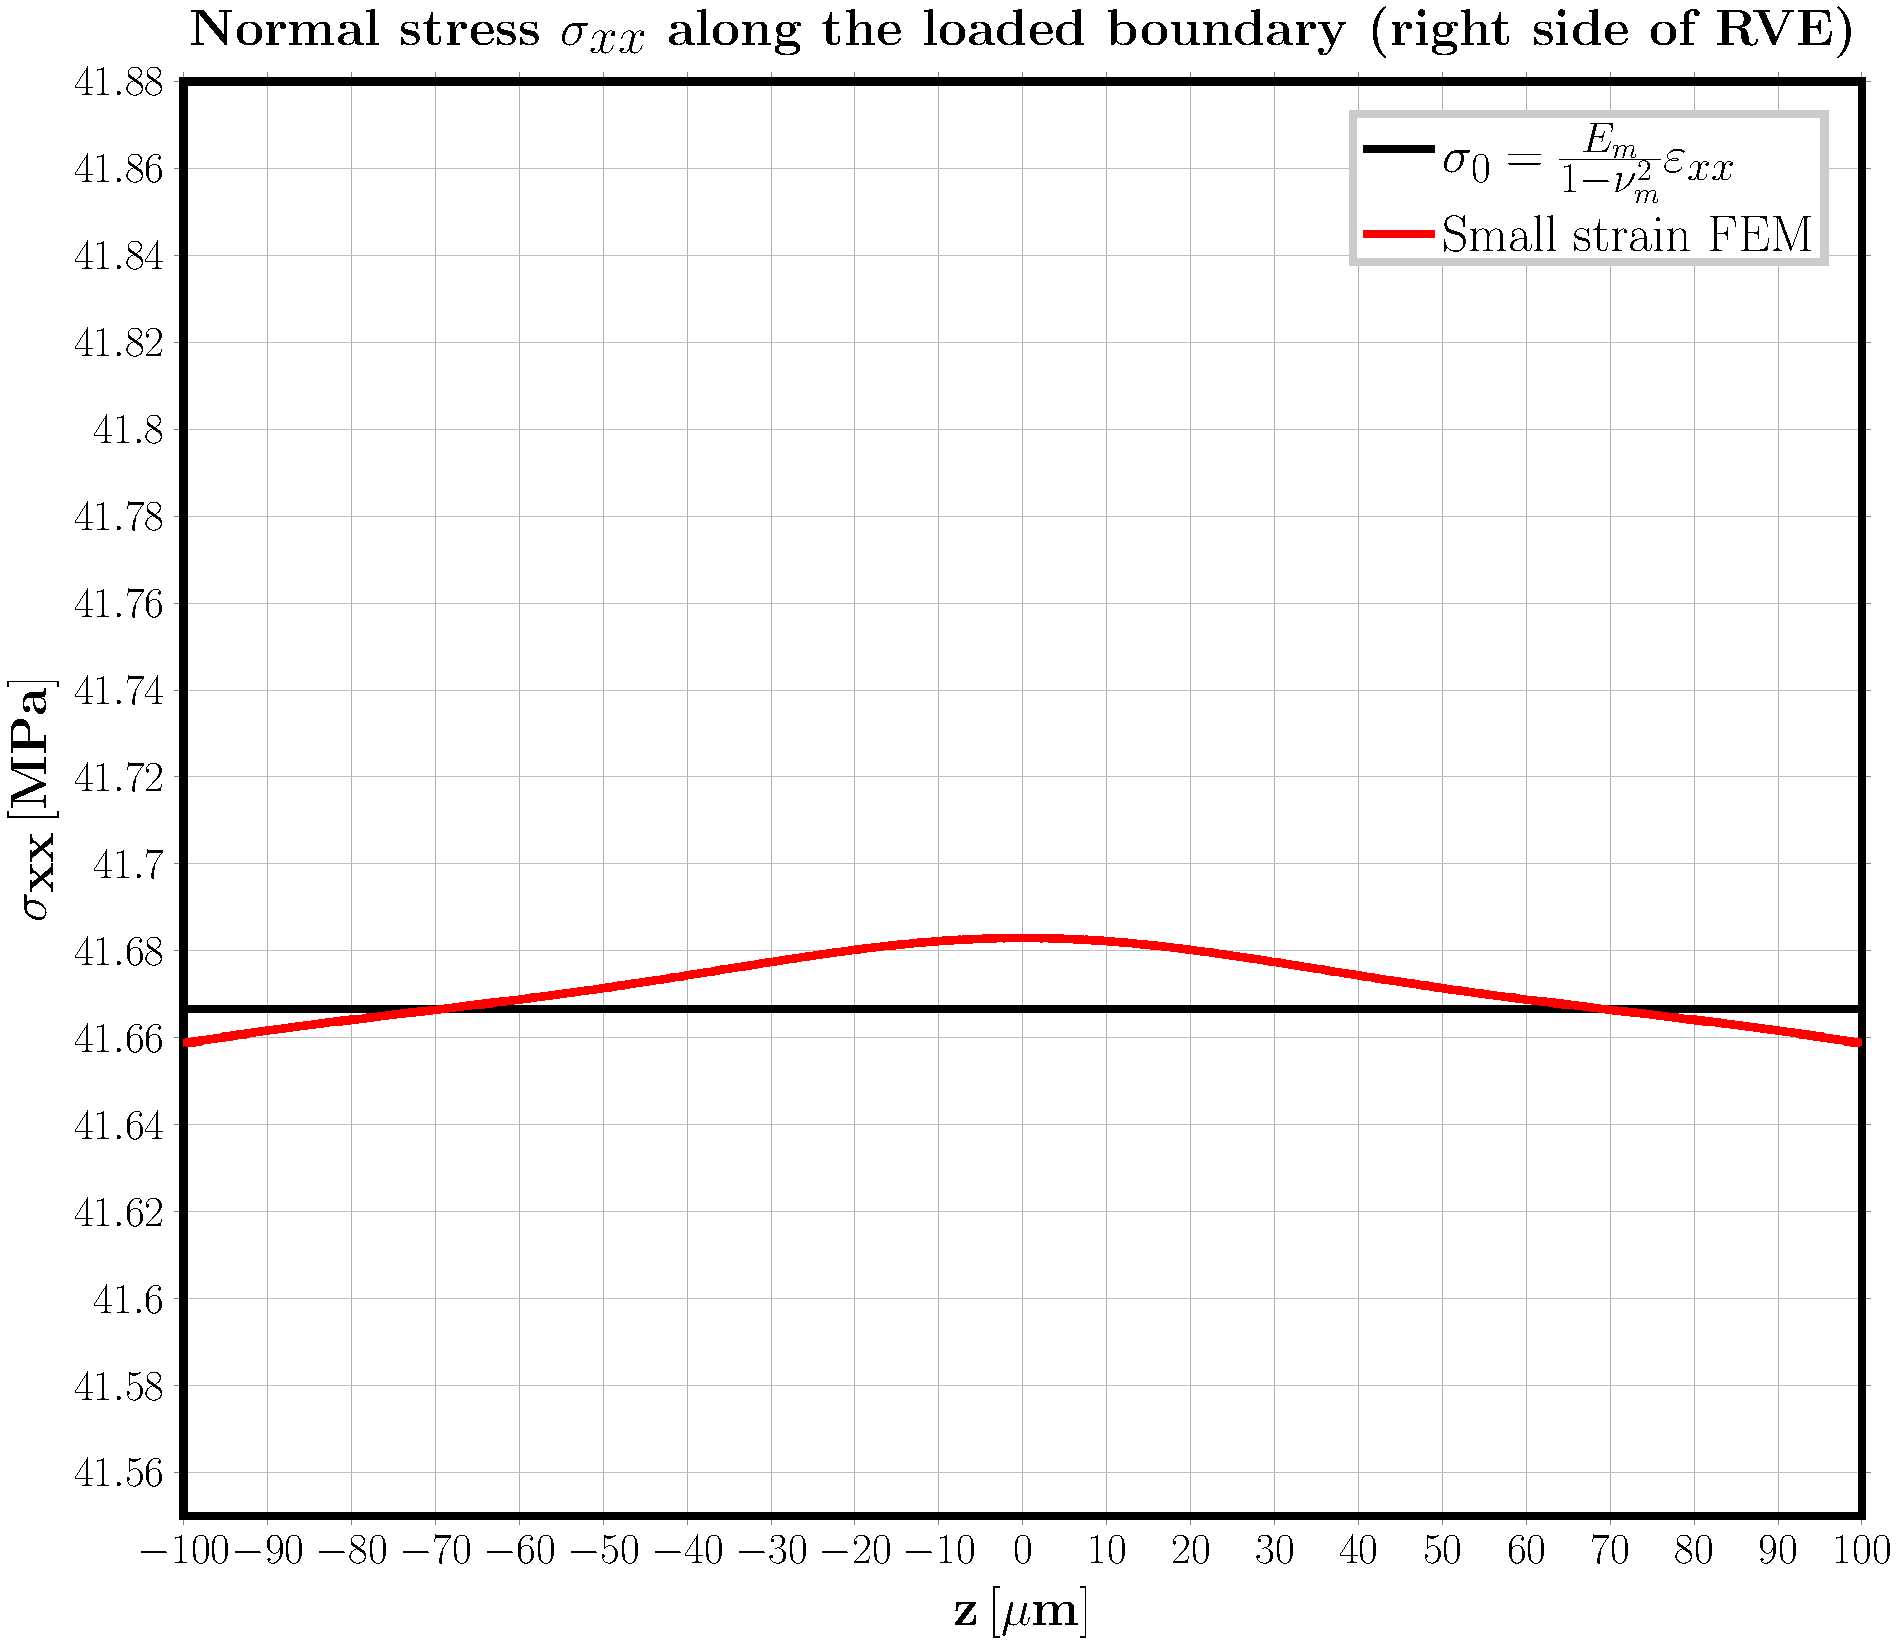
\includegraphics[width=\columnwidth]{2017-06-16_AbqRunSummary_SingleFiberEqRfSmallStrain-D0-4_sigmaatboundary_Summary.pdf}
\caption{\scriptsize  $VF_{f}=0.000079$, $\frac{L}{R_{f}}\sim 100$, $\delta = 0.4^{\circ}$, $\frac{\sigma_{max}-\sigma_{mean}}{\sigma_{mean}}=0.03\%$}
%  \label{fig:jintegral}
\end{figure}
\end{column}
\end{columns}
\end{frame}

\subsection{Normalization $G_{0}$}

\begin{frame}
\frametitle{\small Normalization $G_{0}$ as a function of $\Delta\theta$}
\vspace{-0.5cm}
\centering
\begin{columns}
\begin{column}{0.55\textwidth}
\begin{figure}
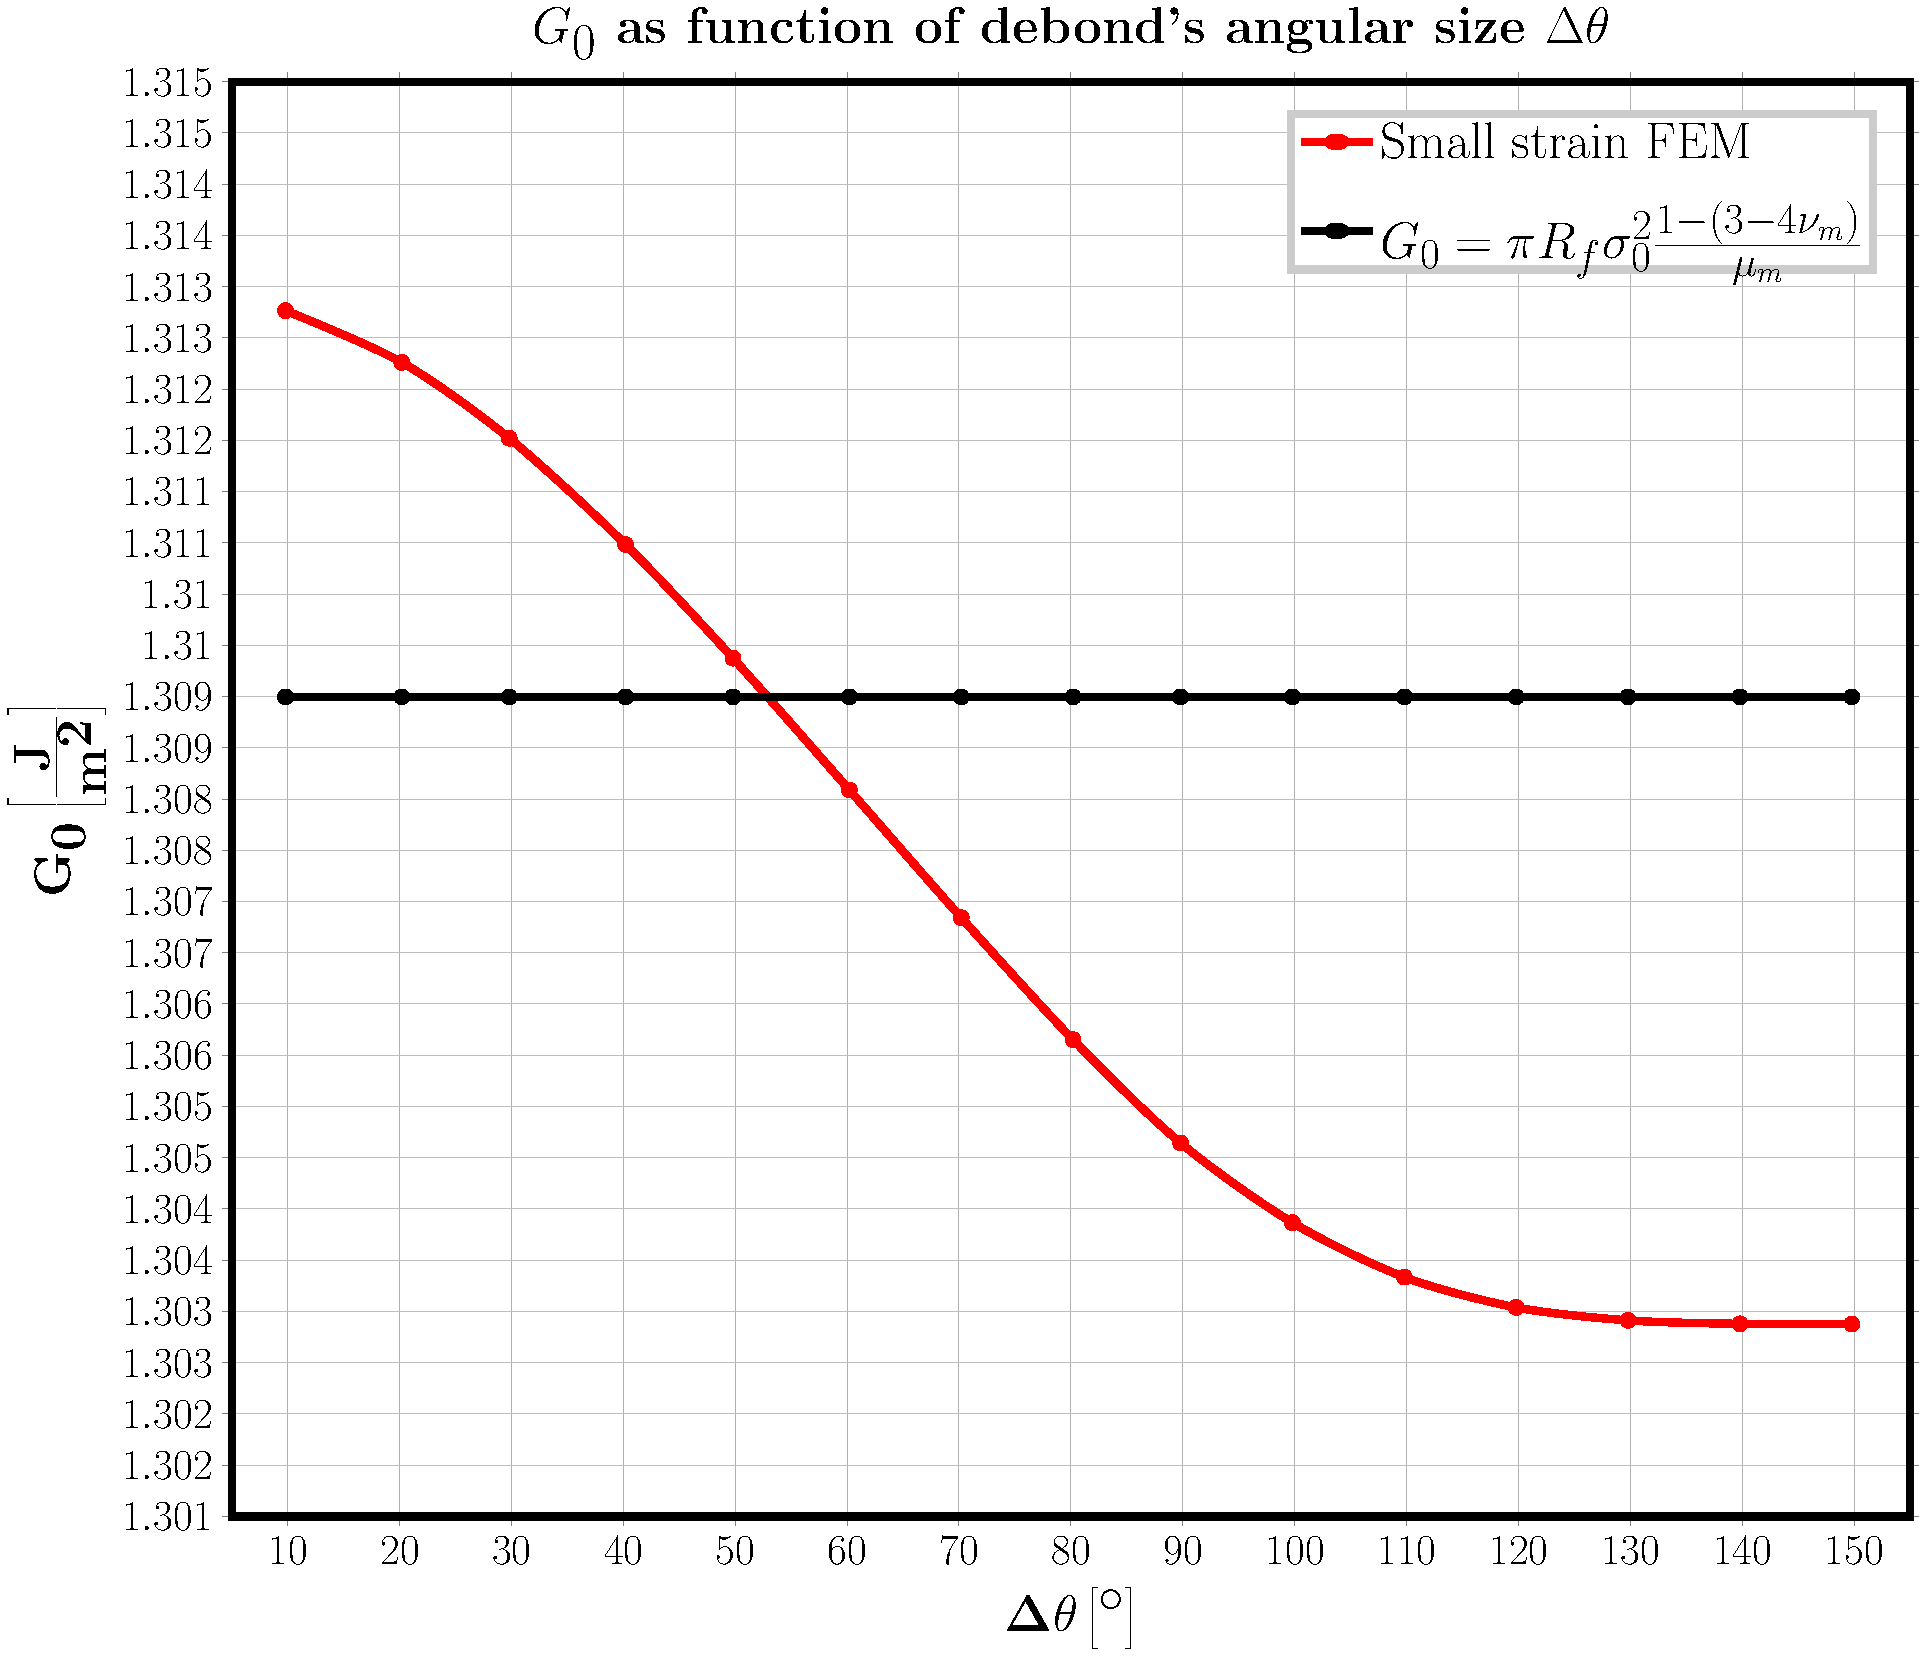
\includegraphics[width=\columnwidth]{2017-06-23_AbqRunSummary_SingleFiberEqRfSmallFiniteStrain_G0_Summary.pdf}
\caption{\scriptsize $VF_{f}=0.001$, $\frac{L}{R_{f}}\sim 28$, $\delta = 0.4^{\circ}$}
%  \label{fig:jintegral}
\end{figure}
\end{column}
\begin{column}{0.55\textwidth}
\begin{figure}
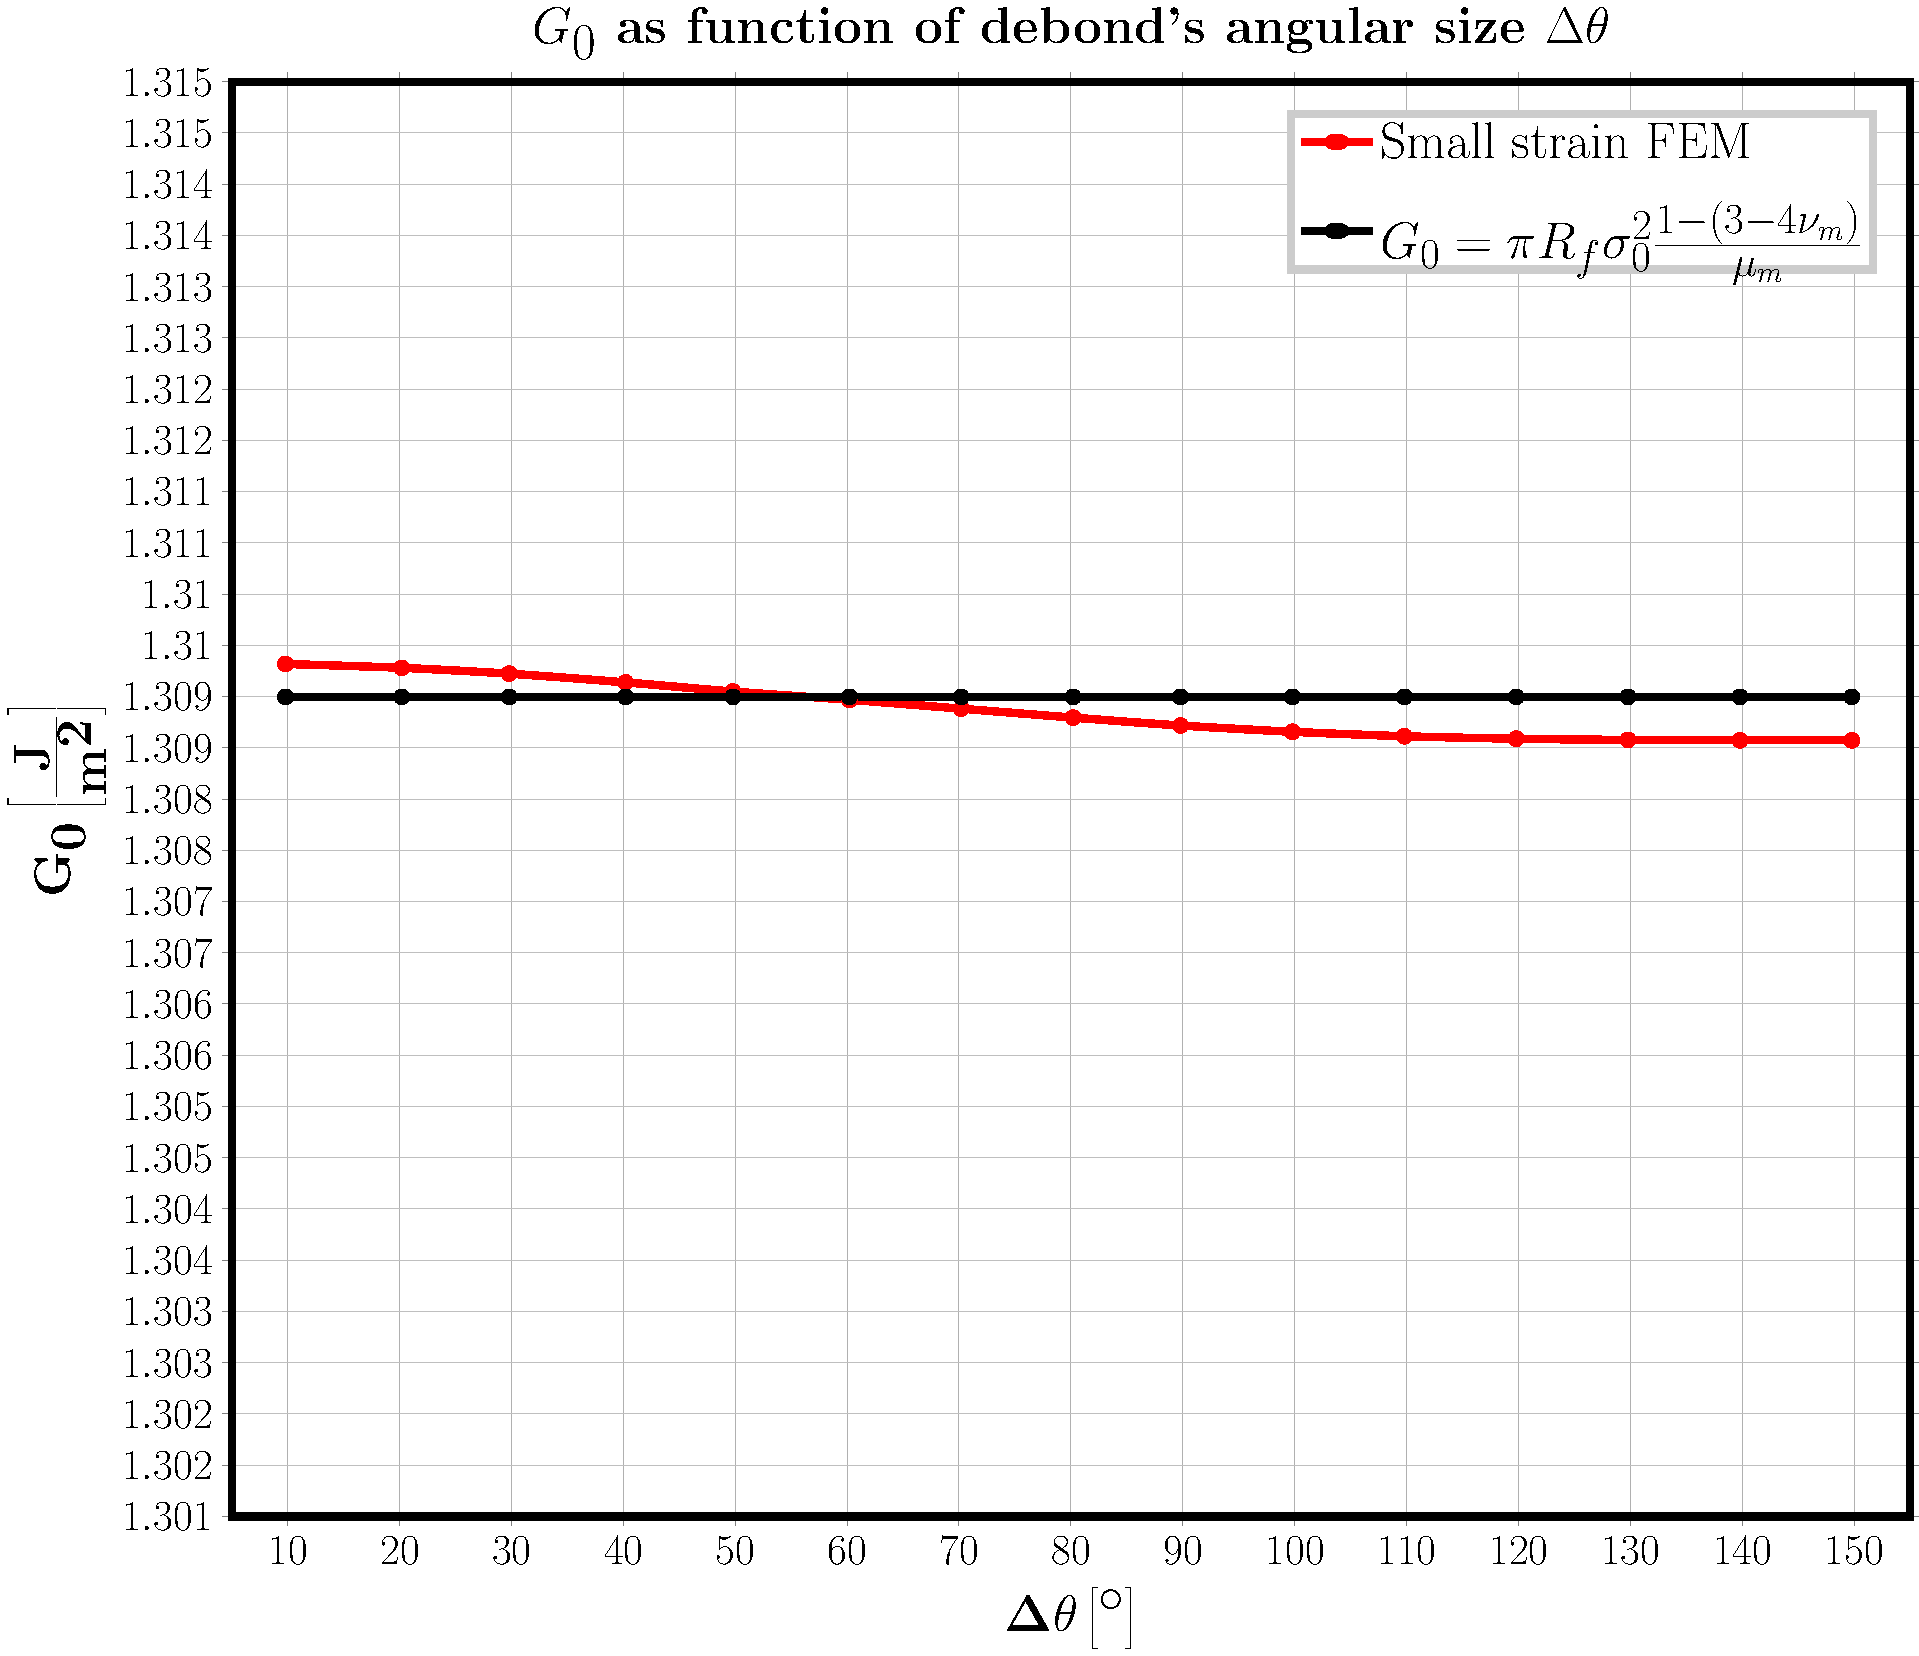
\includegraphics[width=\columnwidth]{2017-06-16_AbqRunSummary_SingleFiberEqRfSmallStrain-D0-4_G0_Summary.pdf}
\caption{\scriptsize  $VF_{f}=0.000079$, $\frac{L}{R_{f}}\sim 100$, $\delta = 0.4^{\circ}$}
%  \label{fig:jintegral}
\end{figure}
\end{column}
\end{columns}
\end{frame}

\subsection{Energy Release Rates}

\begin{frame}
\frametitle{\small Mode I Energy Release Rate $G_{I}$ from VCCT}
\vspace{-0.5cm}
\centering
\captionsetup[figure]{font=scriptsize,labelfont=scriptsize}
\begin{figure}[!h]
\centering
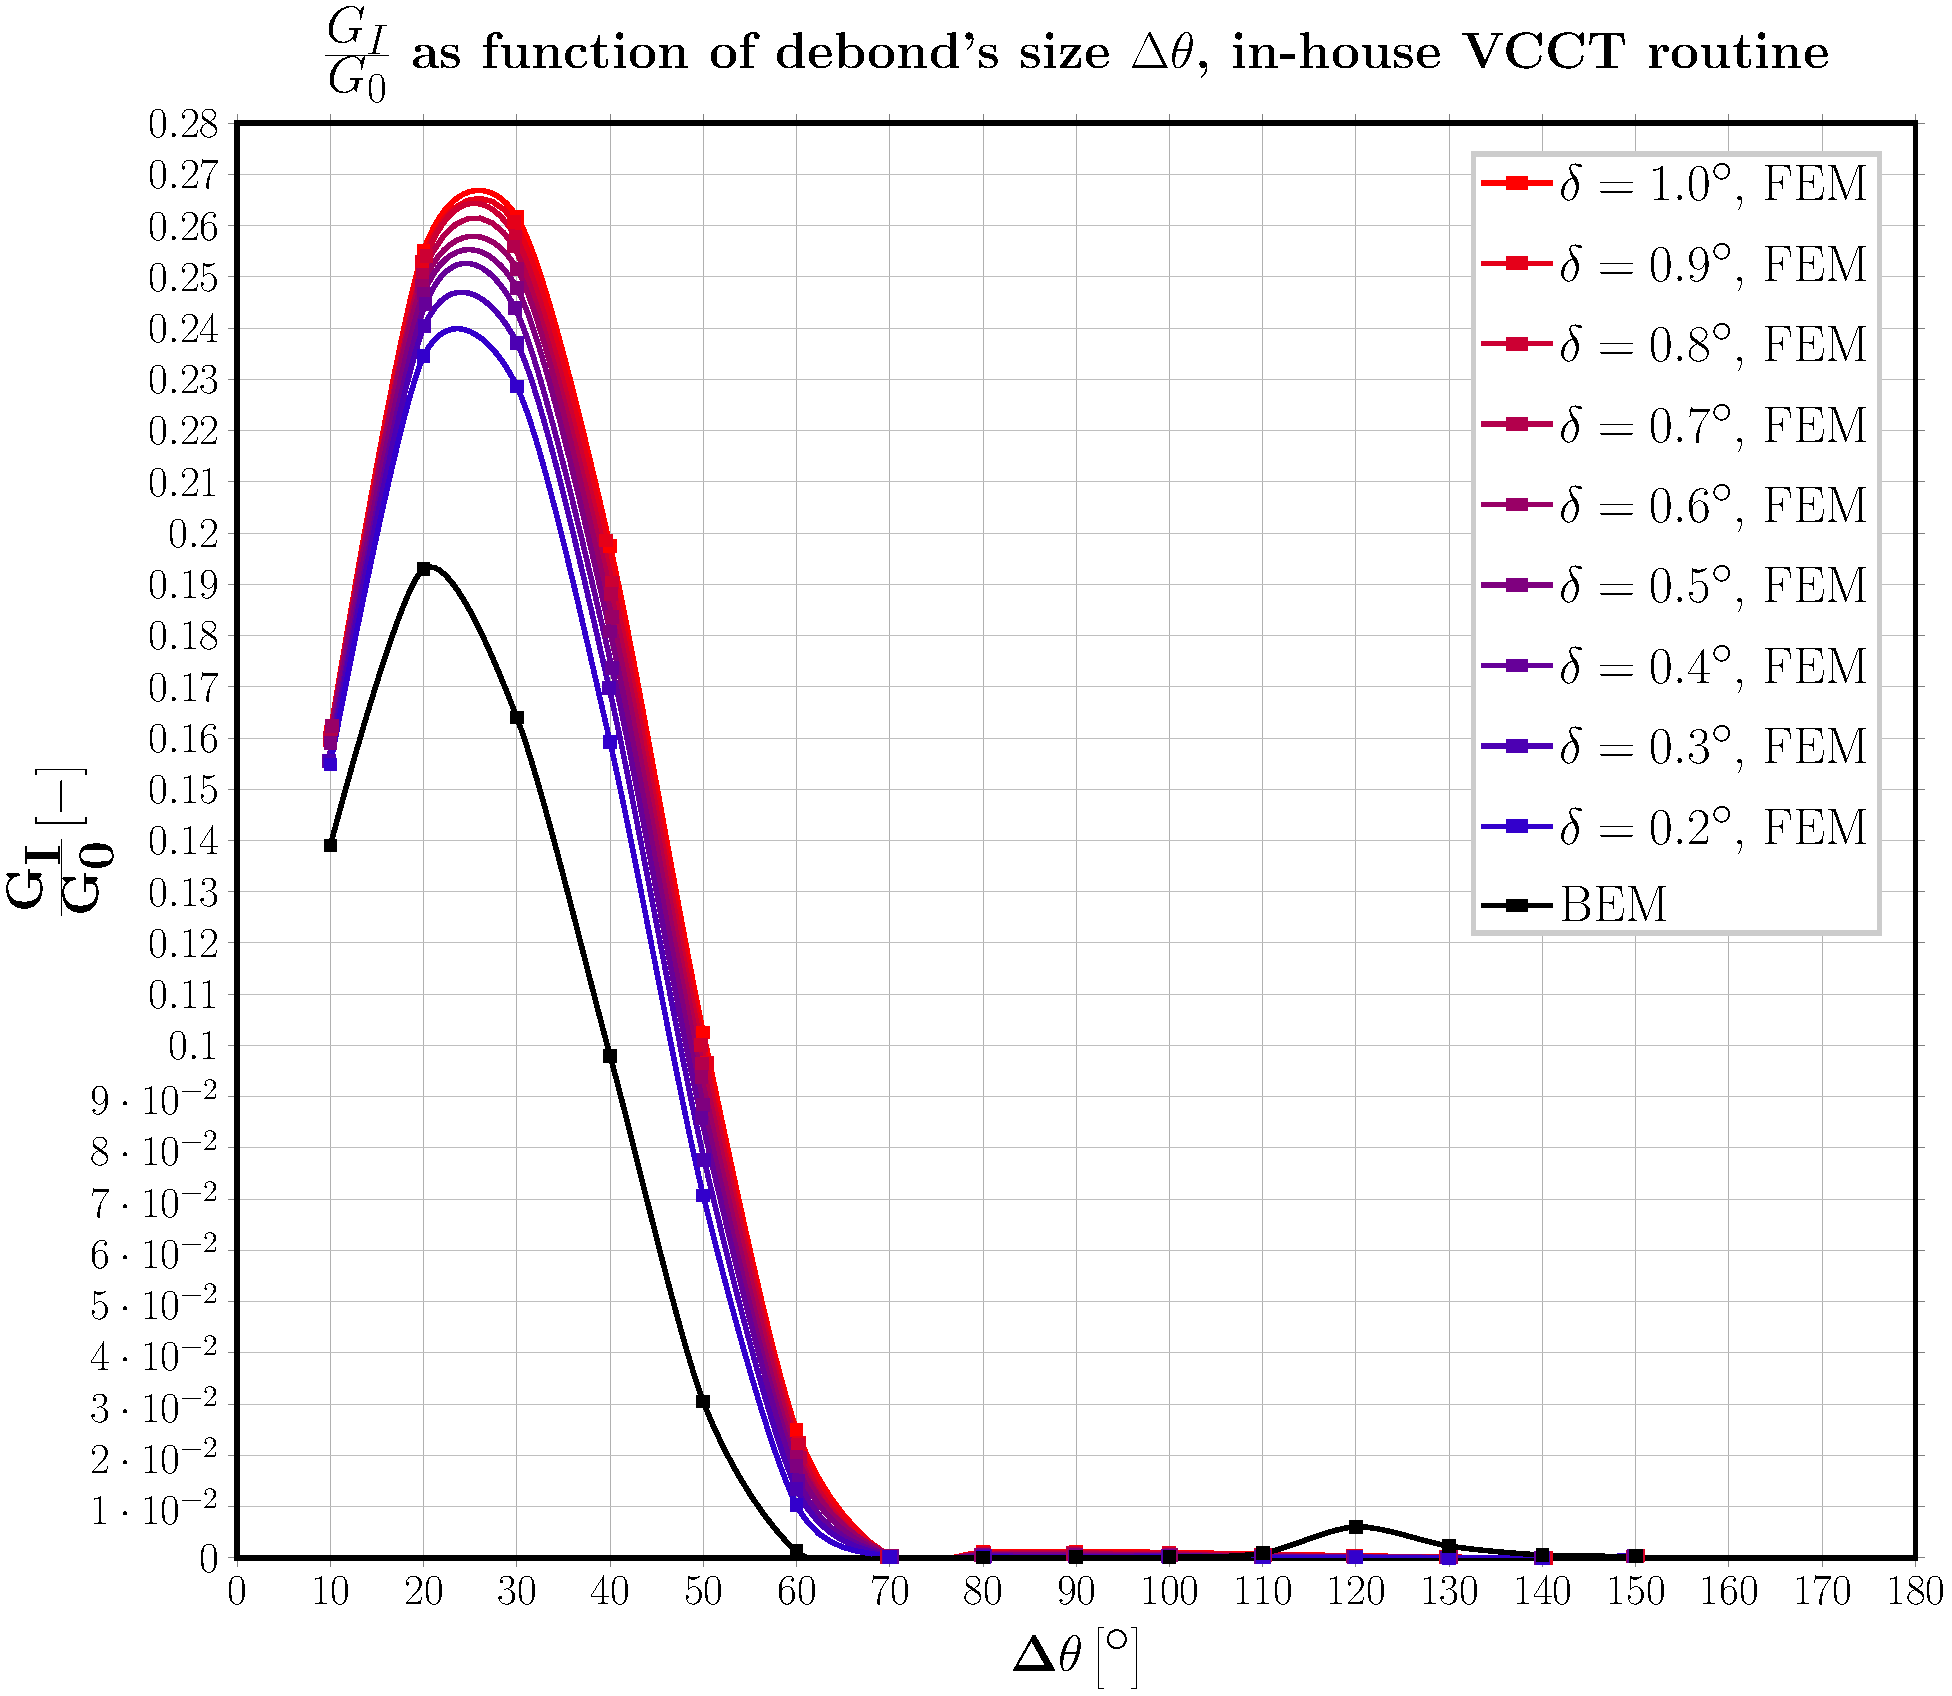
\includegraphics[height=0.7\textheight]{2017-07-10_AbqRunSummary_SmallStrain_M-F-VCCT_GI.pdf}
  \caption{\scriptsize $Vf_{f}=0.000079$, $\frac{L}{R_{f}}\sim 100$; fading from red to blue for decreasing size of elements at the interface, VCCT from FEM results; in black BEM results.}
  \label{fig:res1}
\end{figure}
\end{frame}

\begin{frame}
\frametitle{\small Mode II Energy Release Rate $G_{II}$ from VCCT}
\vspace{-0.5cm}
\centering
\captionsetup[figure]{font=scriptsize,labelfont=scriptsize}
\begin{figure}[!h]
\centering
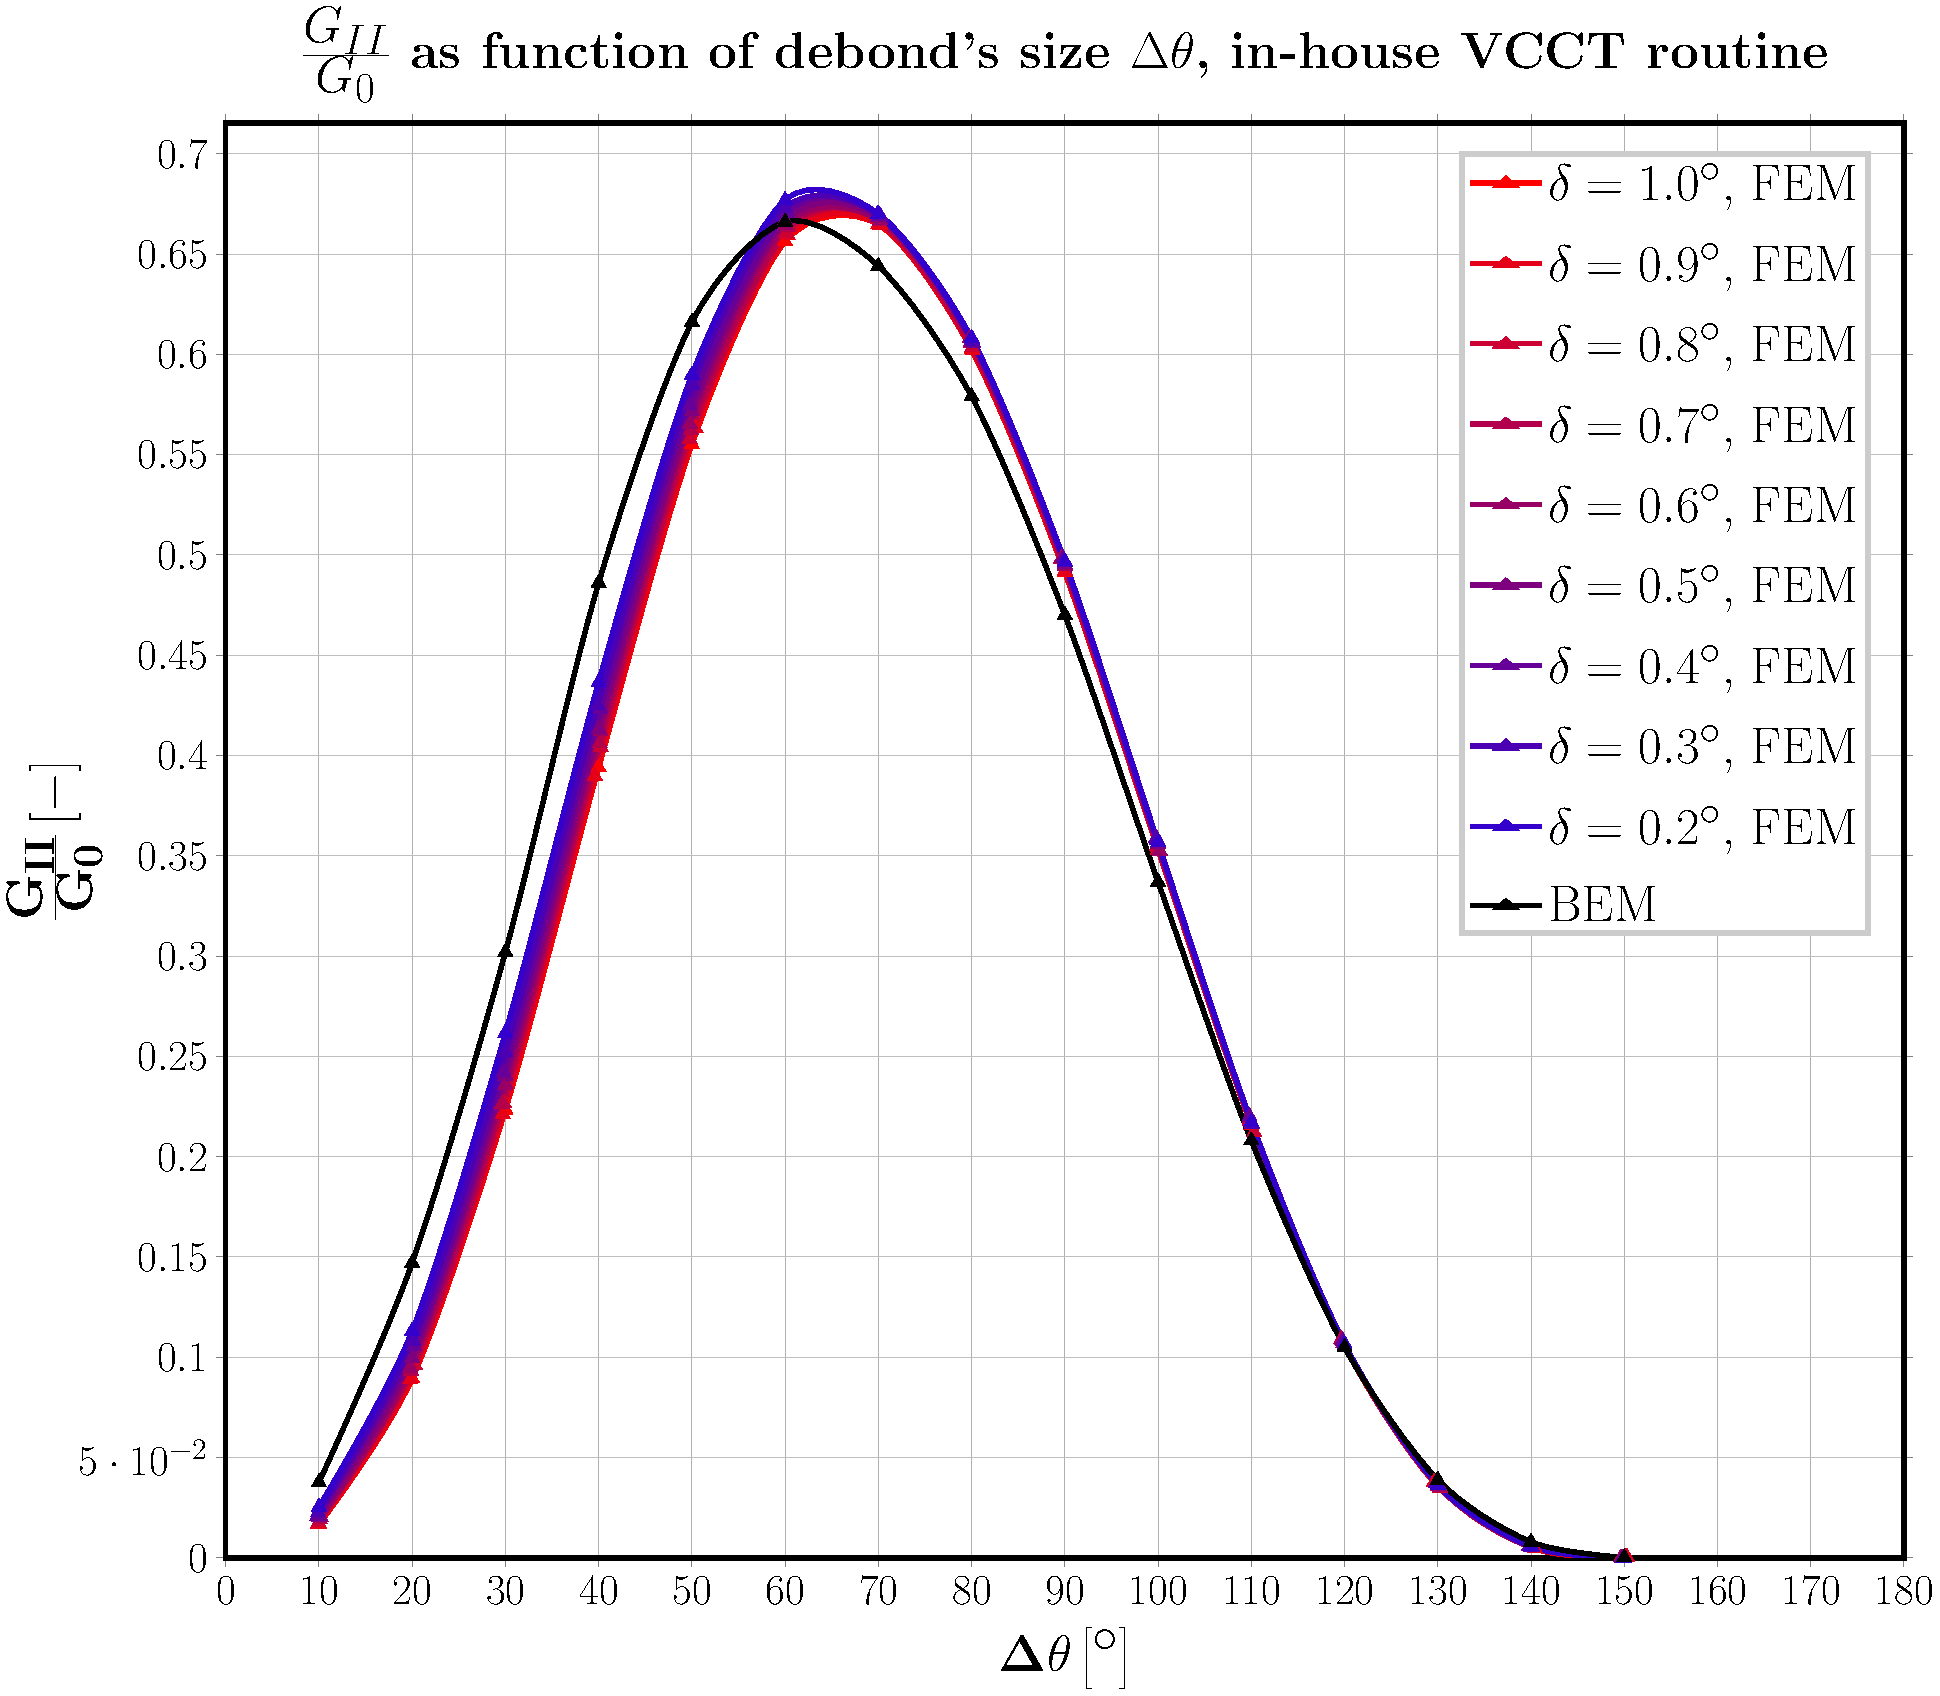
\includegraphics[height=0.7\textheight]{2017-07-10_AbqRunSummary_SmallStrain_M-F-VCCT_GII.pdf}
  \caption{\scriptsize $Vf_{f}=0.000079$, $\frac{L}{R_{f}}\sim 100$; fading from red to blue for decreasing size of elements at the interface, VCCT from FEM results; in black BEM results.}
  \label{fig:res1}
\end{figure}
\end{frame}

\begin{frame}
\frametitle{\small Total Energy Release Rate $G_{TOT}$ from VCCT}
\vspace{-0.5cm}
\centering
\captionsetup[figure]{font=scriptsize,labelfont=scriptsize}
\begin{figure}[!h]
\centering
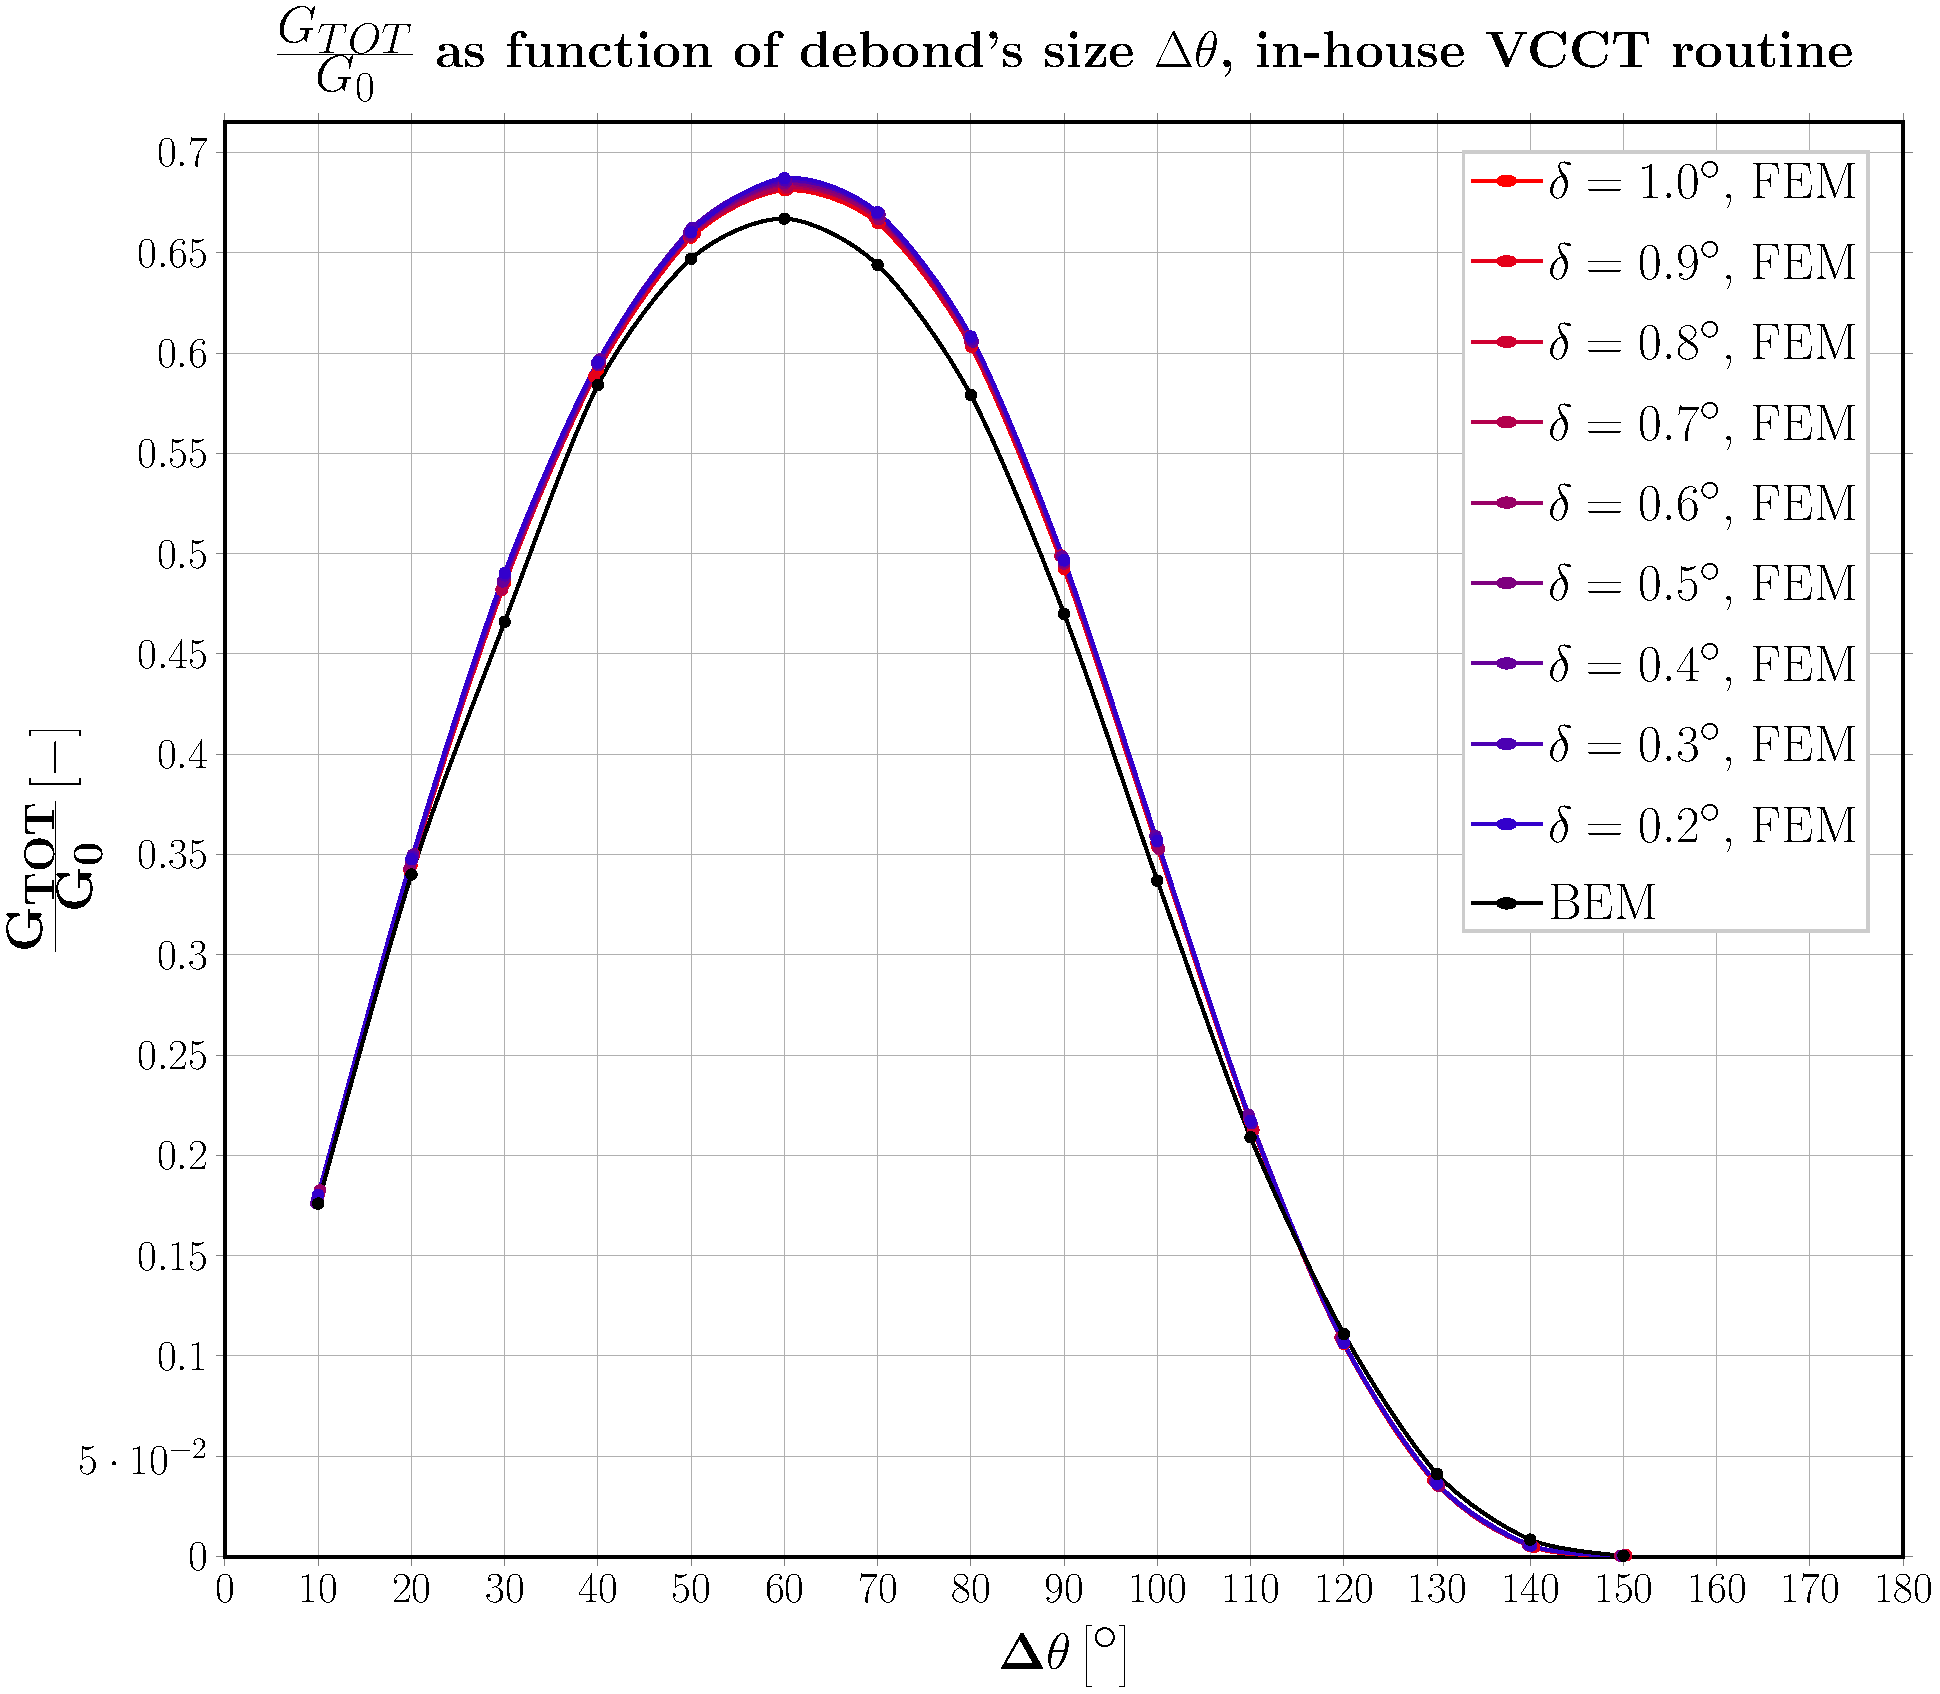
\includegraphics[height=0.7\textheight]{2017-07-10_AbqRunSummary_SmallStrain_M-F-VCCT_GTOT.pdf}
  \caption{\scriptsize $Vf_{f}=0.000079$, $\frac{L}{R_{f}}\sim 100$; fading from red to blue for decreasing size of elements at the interface, VCCT from FEM results; in black BEM results.}
  \label{fig:res1}
\end{figure}
\end{frame}

\section[Conclusions]{Conclusions \& Outlook}

\begin{frame}
\frametitle{\vspace*{0.5cm}\small Conclusions \& Outlook}
\vspace{-0.75cm}
\centering
\scriptsize
\begin{alertblock}{\footnotesize \bf{Conclusions}}
\begin{itemize}[label=\ding{212}]
  \item There is a limiting value of $\frac{L}{R_{f}}$ after which models are effectively infinite
	\item For models larger than this value, domain size and mesh refinement at the interface has a similar effect on the energy release rate
  \item The discrepancy in modes with the use of linear elements might be linked to the deformed shape of crack faces
\end{itemize}
\end{alertblock}
\begin{alertblock}{\footnotesize \bf{Outlook}}
\begin{itemize}[label=\ding{212}]
	\item Modeling extreme ply geometries, for example a ply with a single layer of fibers bounded by stiffer plies\\[9pt]
	\item Investigate the effect of clusters of fibers in thin plies\\[9pt]
	\item Analyzing the effect of complex stress and deformation states, thermal loads, different sets of boundary conditions
\end{itemize}
\end{alertblock}
\end{frame}

\section{Appendices}

\subsection{Timeline}

\begin{frame}
\frametitle{\small Timeline}
\vspace{-0.75cm}
\centering
\scriptsize
\begin{itemize}[label=\ding{212}]
\item Oct. 2015 - Dec. 2017: research in Nancy, FR
\item Jan. 2018 - Dec. 2019: research in Lule\aa, SE\\[20pt]
\item May - June 2016: DocMASE Summer School 2016, Lule\aa, SE; presentation
\item June 2016: quarter-term auto-evaluation report, Nancy, FR
\item April 2017: International Materials Research Meeting of the Greater Region, Sarrebr\"ucken, DE; presentation
\item May 2017: EMMA doctoral school seminar, Nancy, FR; poster
\item July 2017: seminar day of the Research Group 304, Nancy, FR; presentation (in French)
\item October 2017: mid-term defence, Nancy,FR
\item September 2018: mid-term defence, Lule\aa, SE
\item December 2019: doctoral defence, Nancy, FR - Lule\aa, FR
\end{itemize}
\end{frame}

\subsection{Courses \& Training}

\begin{frame}
\frametitle{\small Courses \& Training}
\vspace{-0.75cm}
\centering
\scriptsize
\begin{list}{\Large\textcolor{green}{$\mathbf{\checkmark}$}}{}
\item Scientific courses (40h or 8 ECTS credits)
\item Transverse courses (40h or 8 ECTS credits)
\item Seminars \& Conferences (at least 15 seminars)
\item EMMA seminar (at least 1)
\item Portfolio of competences (regular updates)
\item Quarter-term assessment
\end{list}
\begin{itemize}[label=\ding{212}]
\item Mid-term assessment
\item Doctoriales
\end{itemize}
\end{frame}

%\subsection{Appendices}

%\begin{frame}[label=]
%\frametitle{}
%\end{frame}



%\begin{frame}
%\frametitle{\small Evaluation of $G_{0}$}
%\vspace{-0.7cm}
%\footnotesize
%\centering
%\captionsetup[figure]{font=scriptsize,labelfont=scriptsize}
%\begin{equation}
%G_{0}=\pi R_{f}\sigma^{2}_{0}\frac{1+k_{m}}{8G_{m}}
%\end{equation}
%\begin{equation}
%k_{m}=3-4\nu_{m}
%\end{equation}
%\begin{equation}
%\sigma_{0}^{undamaged}=\frac{E_{m}}{1-\nu^{2}_{m}}\varepsilon_{xx}
%\end{equation}%
%\end{frame}


\subsection{References}

\begin{frame}[allowframebreaks]
  \frametitle{References}

  \begin{thebibliography}{10}

%  \beamertemplatebookbibitems
%  % Start with overview books.
%
%  \bibitem{Author1990}
%    A.~Author.
%    \newblock {\em Handbook of Everything}.
%    \newblock Some Press, 1990.


  \beamertemplatearticlebibitems
  % Followed by interesting articles. Keep the list short.

\bibitem{KawabeTomodaMatsuo:1997} %1
Kawabe K., Tomoda S. and Matsuo T.;
\newblock {\em A pneumatic process for spreading reinforcing fiber tow}
\newblock {\it Proc. 42nd Int. SAMPE USA (Anaheim, CA, USA)} 65–76, 1997.

\bibitem{spreadtowpatent:2003} %2
Kawabe K., Tomoda S.;
\newblock {\em Method of producing a spread multi-filament bundle and an apparatus used in the same.}
\newblock Japan: Fukui Prefectural Government; 2003. JP 2003-193895, 2003.

\bibitem{Kawabe:2008} %3
Kawabe K.;
\newblock {\em New Spreading Technology for Carbon Fiber Tow and Its Application to Composite Materials}
\newblock {\it Sen'i Gakkaishi} {\bf 64} (8) 262--267, 2008 [in Japanese].

\bibitem{SasayamaTomoda:2009} %4
Sasayama H. and Tomoda S.;
\newblock {\em New Carbon Fiber Tow-Spread Technology and Applications to Advanced Composite Materials}
\newblock {\it S.A.M.P.E. journal} {\bf 45} (2) 6--17, 2009.

\bibitem{ntpt} %5
Meijer A.;
\newblock {\em NTPT makes world’s thinnest prepeg even thinner [Internet] [cited 30 April 2017] }
\newblock North Thin Ply Technology (NTPT) press release 2015. Available from http://www.thinplytechnology.com/mesimages/Press\_Release\_NTPT-16JUN2015.pdf.

\bibitem{oxeon} %6
\newblock {\em oXeon TECHNOLOGIES 2014 [Internet] [cited 30 April 2017]}
\newblock Available from http://oxeon.se/technologies/.

\bibitem{DonaldL.Flaggs1982}  %7
Donald L. Flaggs, Murat H. Kural;
\newblock {\em Experimental Determination of the In Situ Transverse Lamina Strength in Graphite/Epoxy Laminates.}
\newblock {\it J. Comp. Mat.} {\bf 16} 2, 1982.

\bibitem{Krueger:2004}  %8
Krueger R.;
\newblock {\em Virtual crack closure technique: History, approach, and applications}
\newblock {\it Appl. Mech. Rev.} {\bf 57} (2) 109--143, 2004.

\bibitem{Rice:1968}  %9
Rice J. R.;
\newblock {\em A Path Independent Integral and the Approximate Analysis of Strain Concentration by Notches and Cracks}
\newblock {\it J. Appl. Mech.} {\bf 35} 379--386, 1968.

\bibitem{Toya:1975}  %10
Toya M.;
\newblock {\em A Crack Along the Interface of a Circular Inclusion Embedded in an Infinite Solid}
\newblock {\it J. Mech. Phys.} {\bf 22} 325--348, 1975.

\bibitem{Paris:1996}  %11
Par\'is F., Ca\~no J. C., Varna J.;
\newblock {\em The fiber-matrix interface crack - A numerical analysis using Boundary Elements}
\newblock {\it Int. J. Fract.} {\bf 82} 1 11--29, 1996.

  \end{thebibliography}
\end{frame}

\begin{frame}[plain]
\frametitle{}
\end{frame}

\end{document}
